\documentclass[14pt]{book}

\usepackage{fancyhdr}
\usepackage{graphicx}
\usepackage[margin=2.5cm]{geometry}
\usepackage{graphicx}
\usepackage{anysize}
\usepackage{xcolor}
\usepackage{caption}
\usepackage{subcaption}

\marginsize{2cm}{2cm}{2cm}{2cm} % Izquierda, derecha, arriba, abajo
\setlength{\parindent}{0cm}
\pagestyle{fancy}
\fancyhf{}
\fancyhead[L]{\footnotesize Redes de computadoras} %encabezado izquierda
\fancyhead[R]{\footnotesize David Pérez Jacome}   % derecha
\fancyfoot[L]{\footnotesize}  %izquierda
\fancyfoot[C]{Página \thepage}
\renewcommand{\footrulewidth}{0.4pt}

\begin{document}
\begin{center}
  \newcommand{\HRule}{\rule{\linewidth}{0.5mm}}
  \begin{minipage}{0.48\textwidth}
    \begin{flushleft}
      
\includegraphics[scale = 0.08]{images/logo_unam.png}
    \end{flushleft}
  \end{minipage}
  \begin{minipage}{0.48\textwidth}
    \begin{flushright}
      
\includegraphics[scale =0.22]{images/logo_ciencias.png}
    \end{flushright}
  \end{minipage}
  \vspace*{-1.5cm}
  \textsc{\huge Nacional Autónoma de México \\ \vspace{-4px} Universidad }\\[2cm]
  \textsc{\LARGE Facultad de Ciencias}\\[1.5cm]
  \begin{minipage}{0.9\textwidth}
    \begin{center}
      \textsc{\LARGE Redes de computadoras}
    \end{center}
  \end{minipage}\\[0.5cm]
  \vspace*{1cm}
  \HRule \\[0.4cm]
  { \huge \bfseries Practica 07}\\[0.4cm]
  \HRule \\[1.5cm]
  \begin{minipage}{0.52\textwidth}
    \begin{flushleft} \large \small \vspace{-0.6cm} \vspace{-0.6cm}
      Alumno David Pérez Jacome \\
    \end{flushleft}
  \end{minipage}
  \begin{minipage}{0.46\textwidth}
    \vspace{-0.6cm}
    \begin{flushright} \large \small \emph{Profesor:}
      Paulo Santiago de Jesús Contreras Flores \\
    \end{flushright}
  \end{minipage}
  \vspace*{1cm}
  \vspace{2cm}
  \begin{center}
    {\large 2023}
  \end{center}
\end{center}
\newpage

{\color{blue} \section*{\textbf{Practica 07}}}
\vspace{1em}

{\color{red} \subsection*{\textbf{Ruteo dinámico con OSPF}}}
\vspace{1em}

{\color{red} \subsection*{\textbf{Objetivo}}}
\vspace{1em}

\begin{enumerate}
  \item El alumno aprenderá el uso del software de simulación de redes Packet Tracer.
  \item Configurará rutas dinámicas usando el protocolo OSPF, en los router de diferentes redes.
  \item Configurará un router para el intercambio de información de rutas entre los protocolos RIP y OSPF.
\end{enumerate}

{\color{red} \subsection*{\textbf{Introducción}}}
\vspace{1em}

El protocolo OSPF (Open Shortest Path First) es un protocolo de ruteo que utiliza el algoritmo de
estado de enlace para la distribución y cálculo de rutas, se desarrolló como reemplazo del protocolo
RIP del tipo vector de distancias. OSPF presenta ventajas importantes en comparación con RIP,
ya que ofrece una convergencia más rápida y un mejor desempeño en redes de mayor tamaño.\\

{\color{red} \subsection*{\textbf{Desarrollo}}}
\vspace{1em}

{\color{blue} \subsubsection*{\textbf{Configuración de rutas dinámicas usando OSPF}}}
\vspace{1em}

Primero vamos a borrar la configuración previa del protocolo RIP, ya que ahora se usarán rutas dinámicas usando el
protocolo OSPF.\\

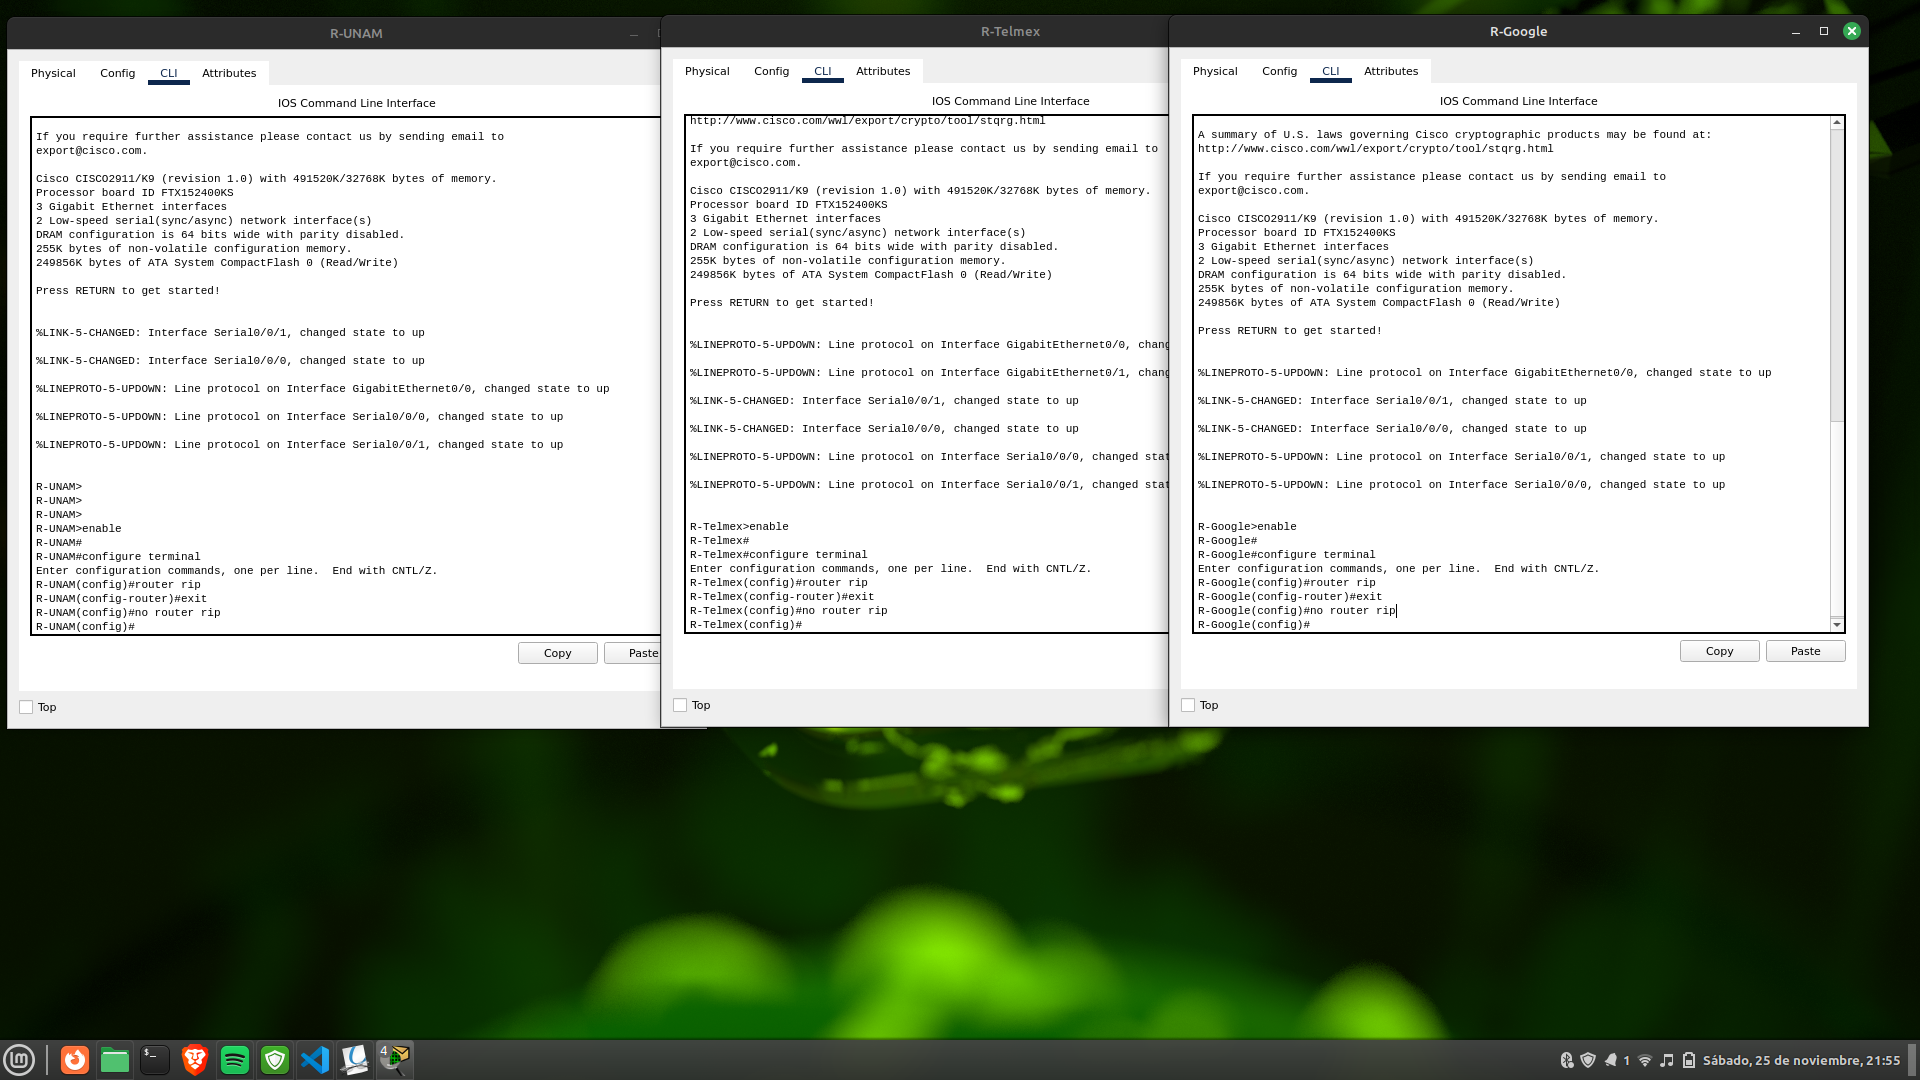
\includegraphics[width=12cm, height=8cm]{images/no router rip.png}\\

Despues en el router-UNAM reconfiguramos las rutas dinámicas
usando el protocolo RIP. Además de que se redistribuirá las rutas hacia la interfaz que esté
configurada con el protocolo OSPF.\\

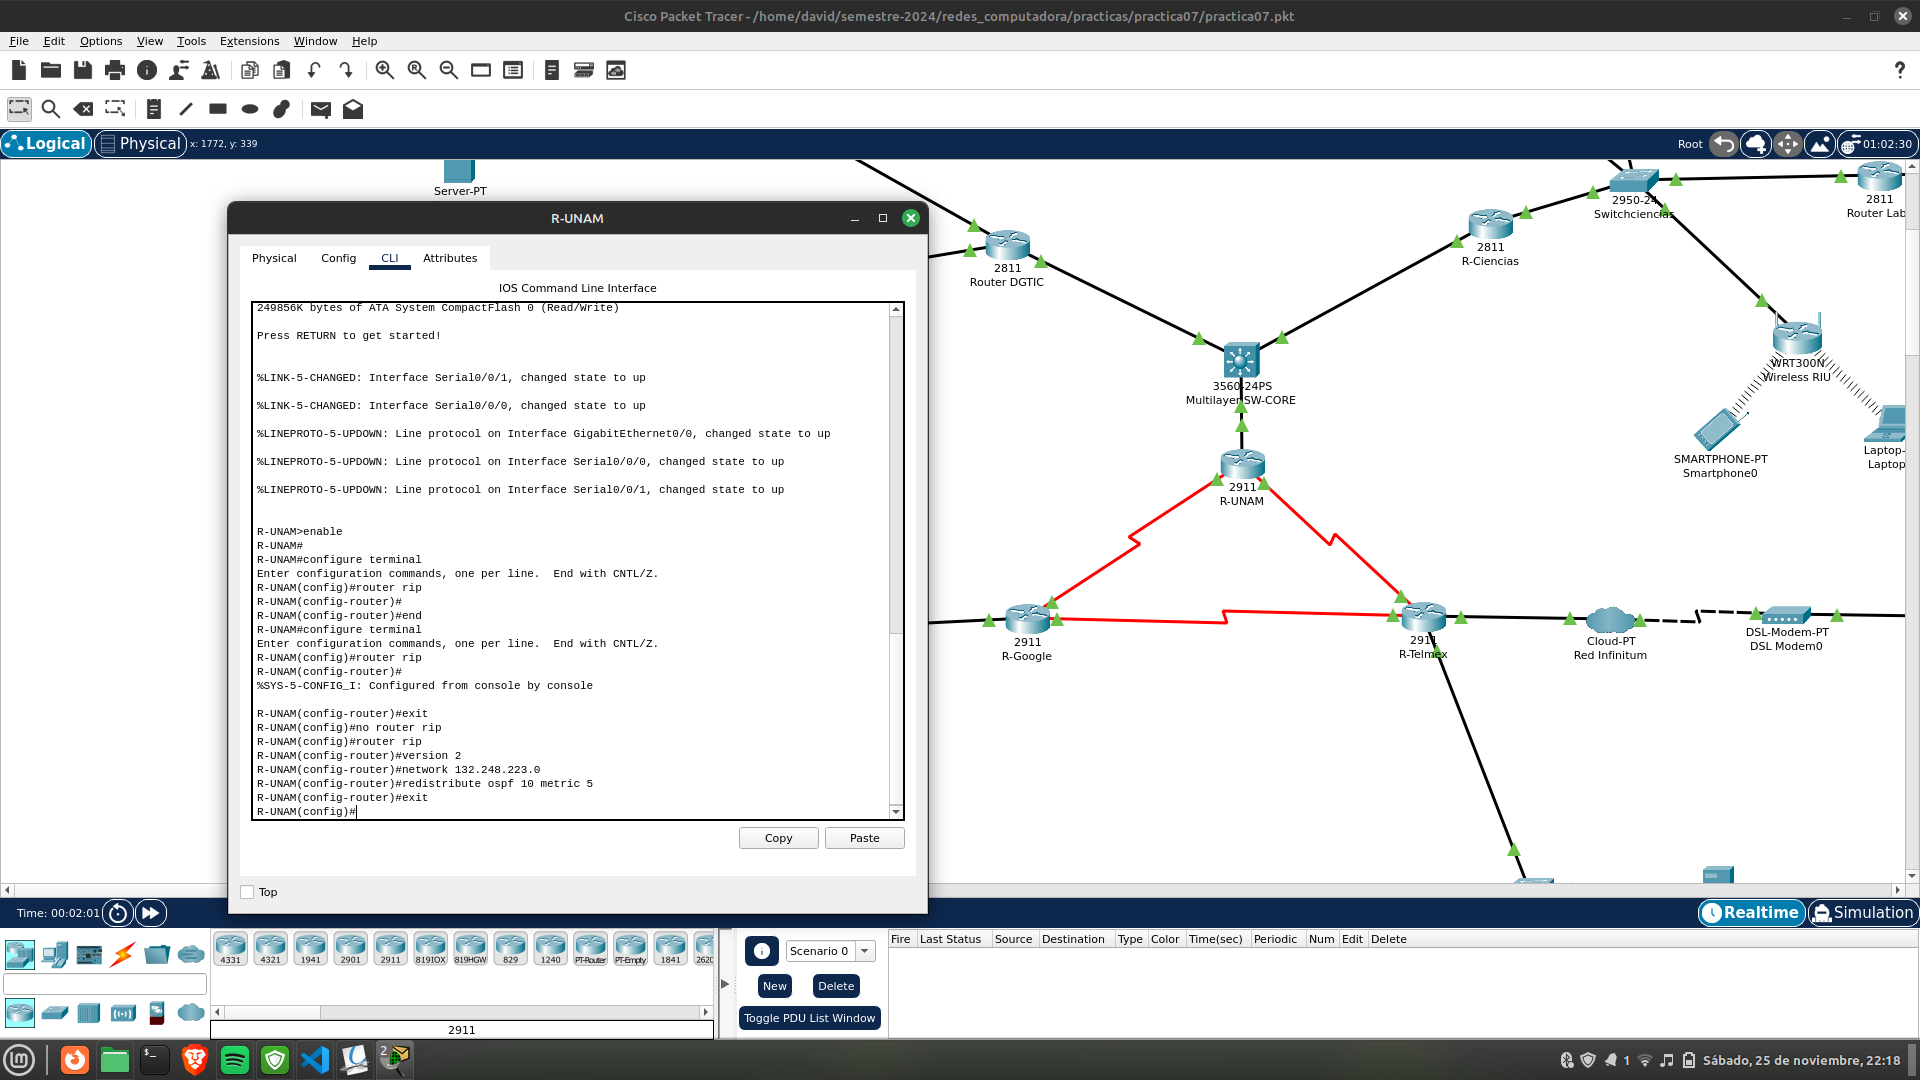
\includegraphics[width=12cm, height=8cm]{images/configuracion unam 2.png}\\

Despues primero en el router UNAM configuramos las rutas dinámicas
usando el protocolo OSPF\\

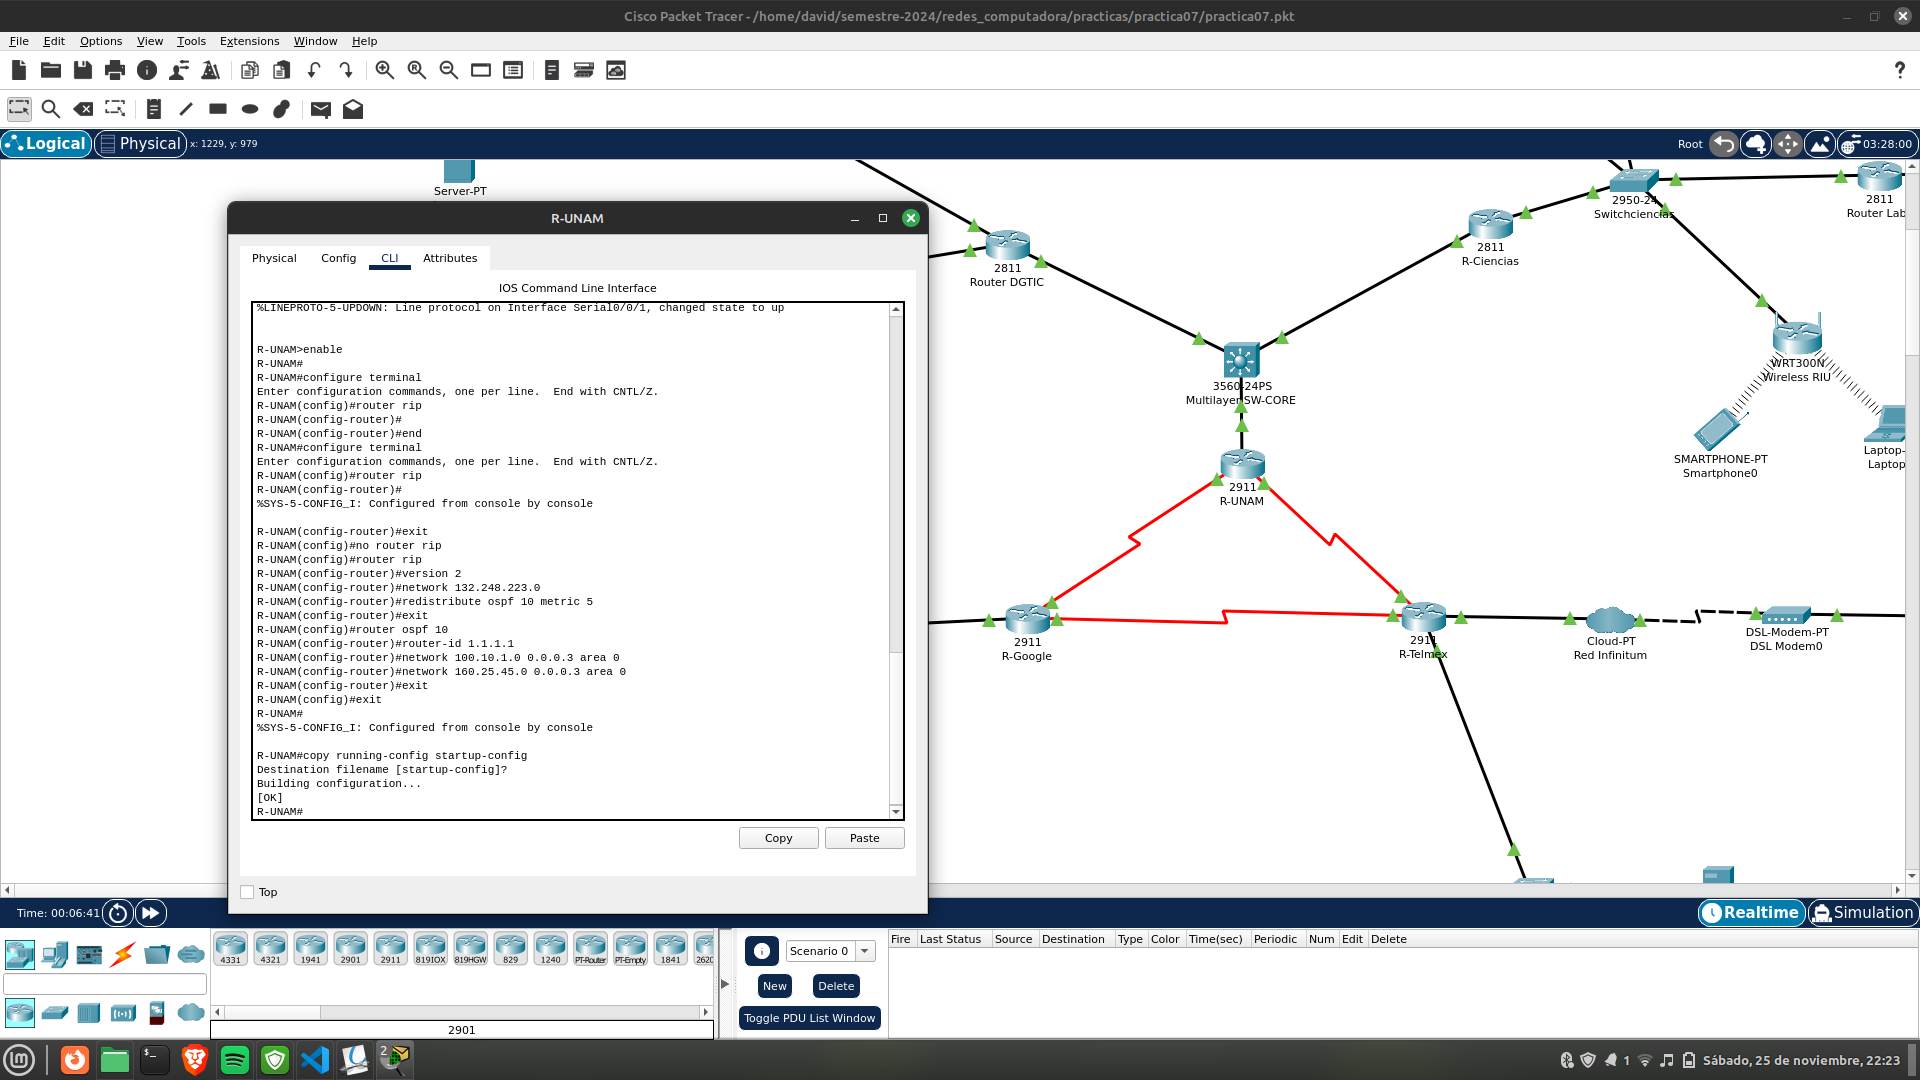
\includegraphics[width=12cm, height=8cm]{images/configutacion general 1.png}\\

Seguido lo hacemos con el Router Google.\\
 
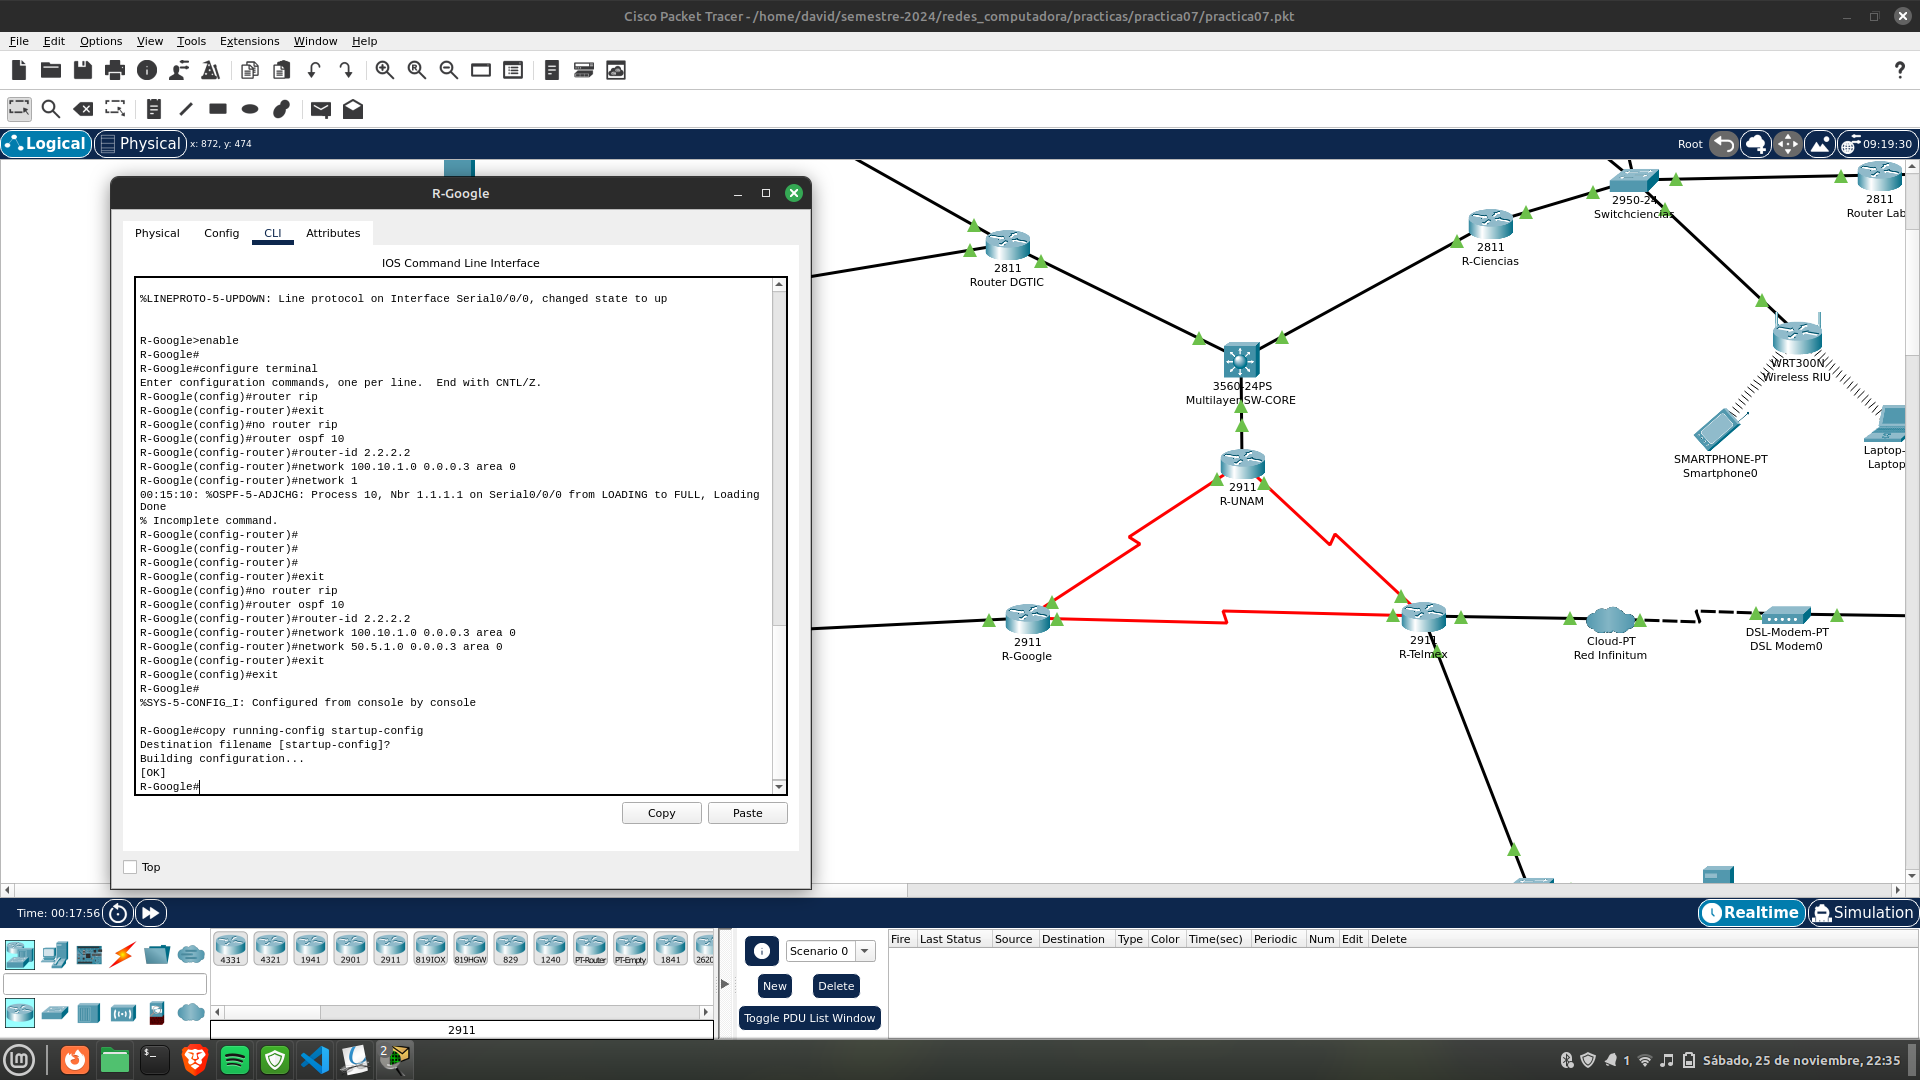
\includegraphics[width=12cm, height=8cm]{images/general google.png}\\

Y terminamos con el router Telmex\\

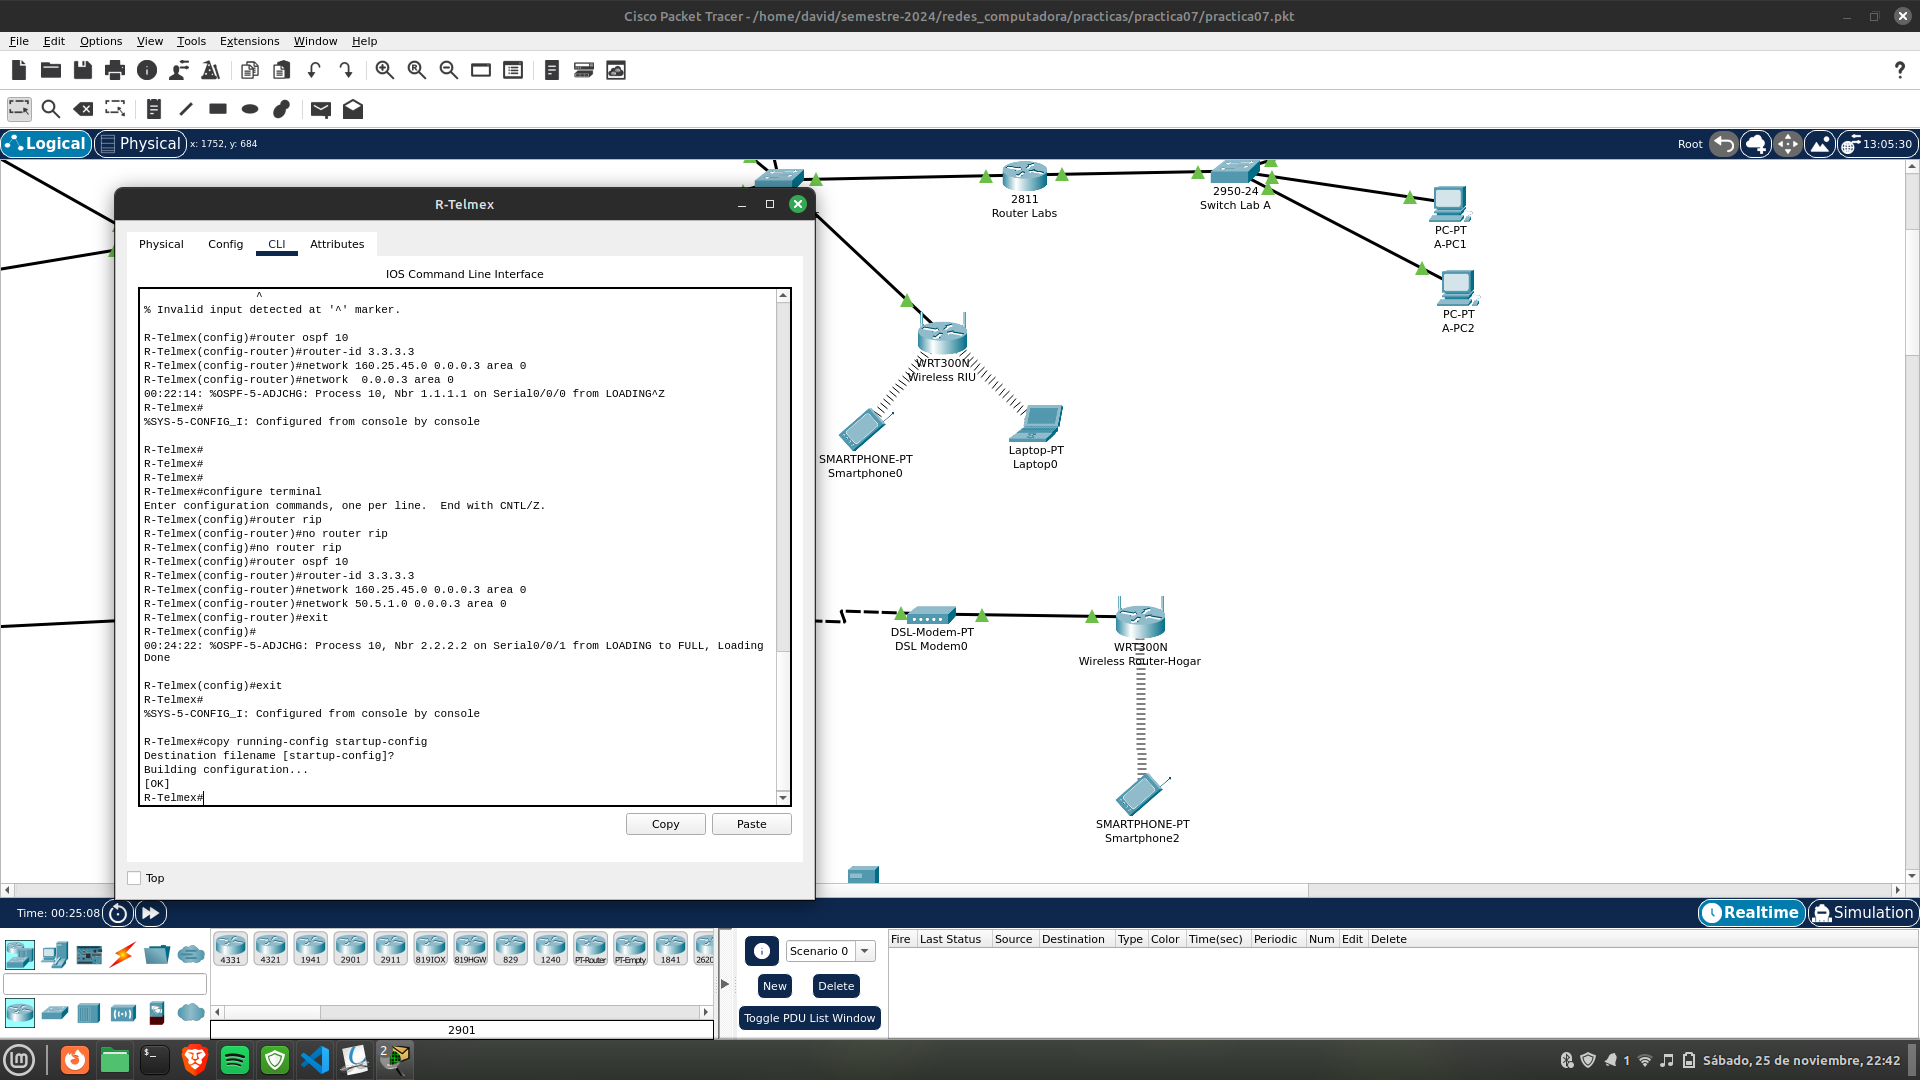
\includegraphics[width=12cm, height=8cm]{images/general telmex.png}\\

Despues redistribuimos las rutas entre los Router DGTIC y Ciencias, y el SW-Core que utilizan RIP, hacia la interfaz de red del Router
UNAM que usa junto con el resto de los Router, al protocolo OSPF.\\

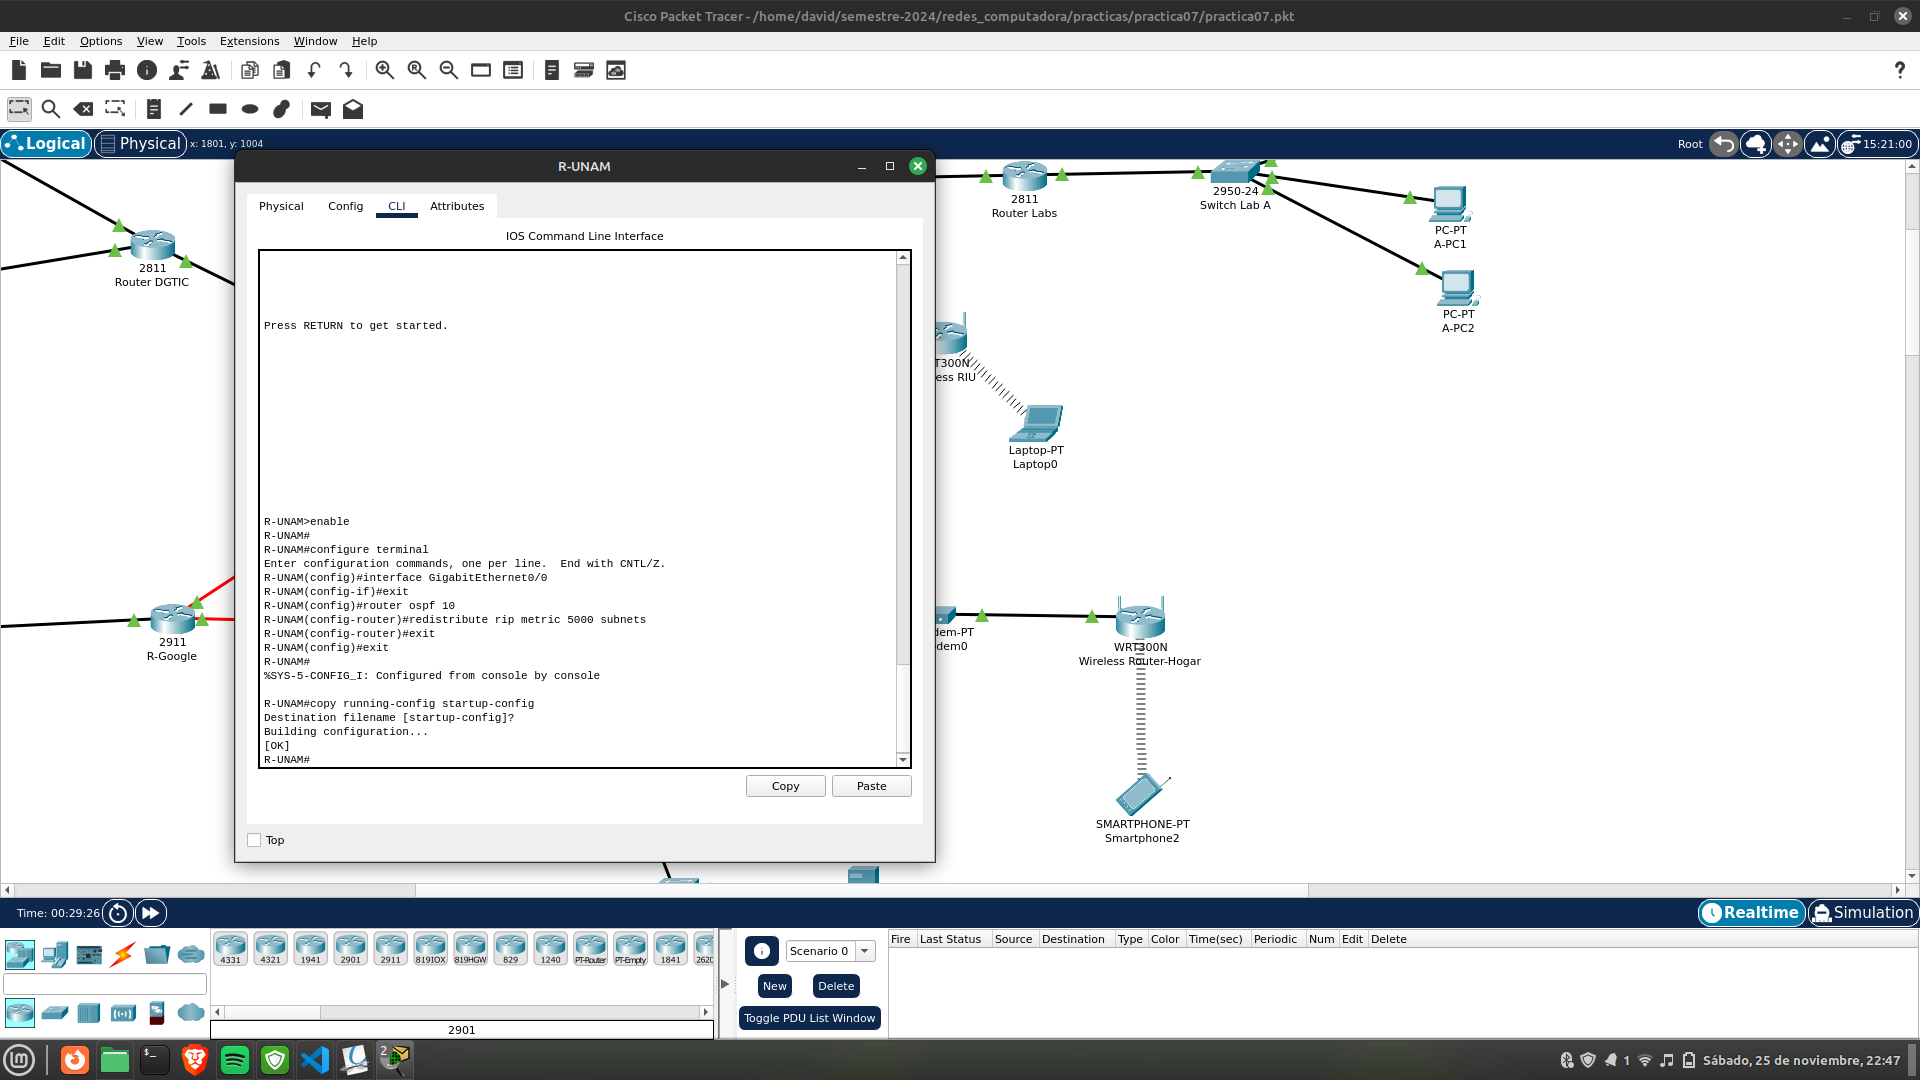
\includegraphics[width=12cm, height=8cm]{images/redistro unam.png}\\

{\color{blue} \subsubsection*{\textbf{Comprobar la configuración}}}
\vspace{1em}

Mostraremos la configuración de los siguientes comandos para los Router UNAM, Google y
Telmex\\

Para UNAM:\\

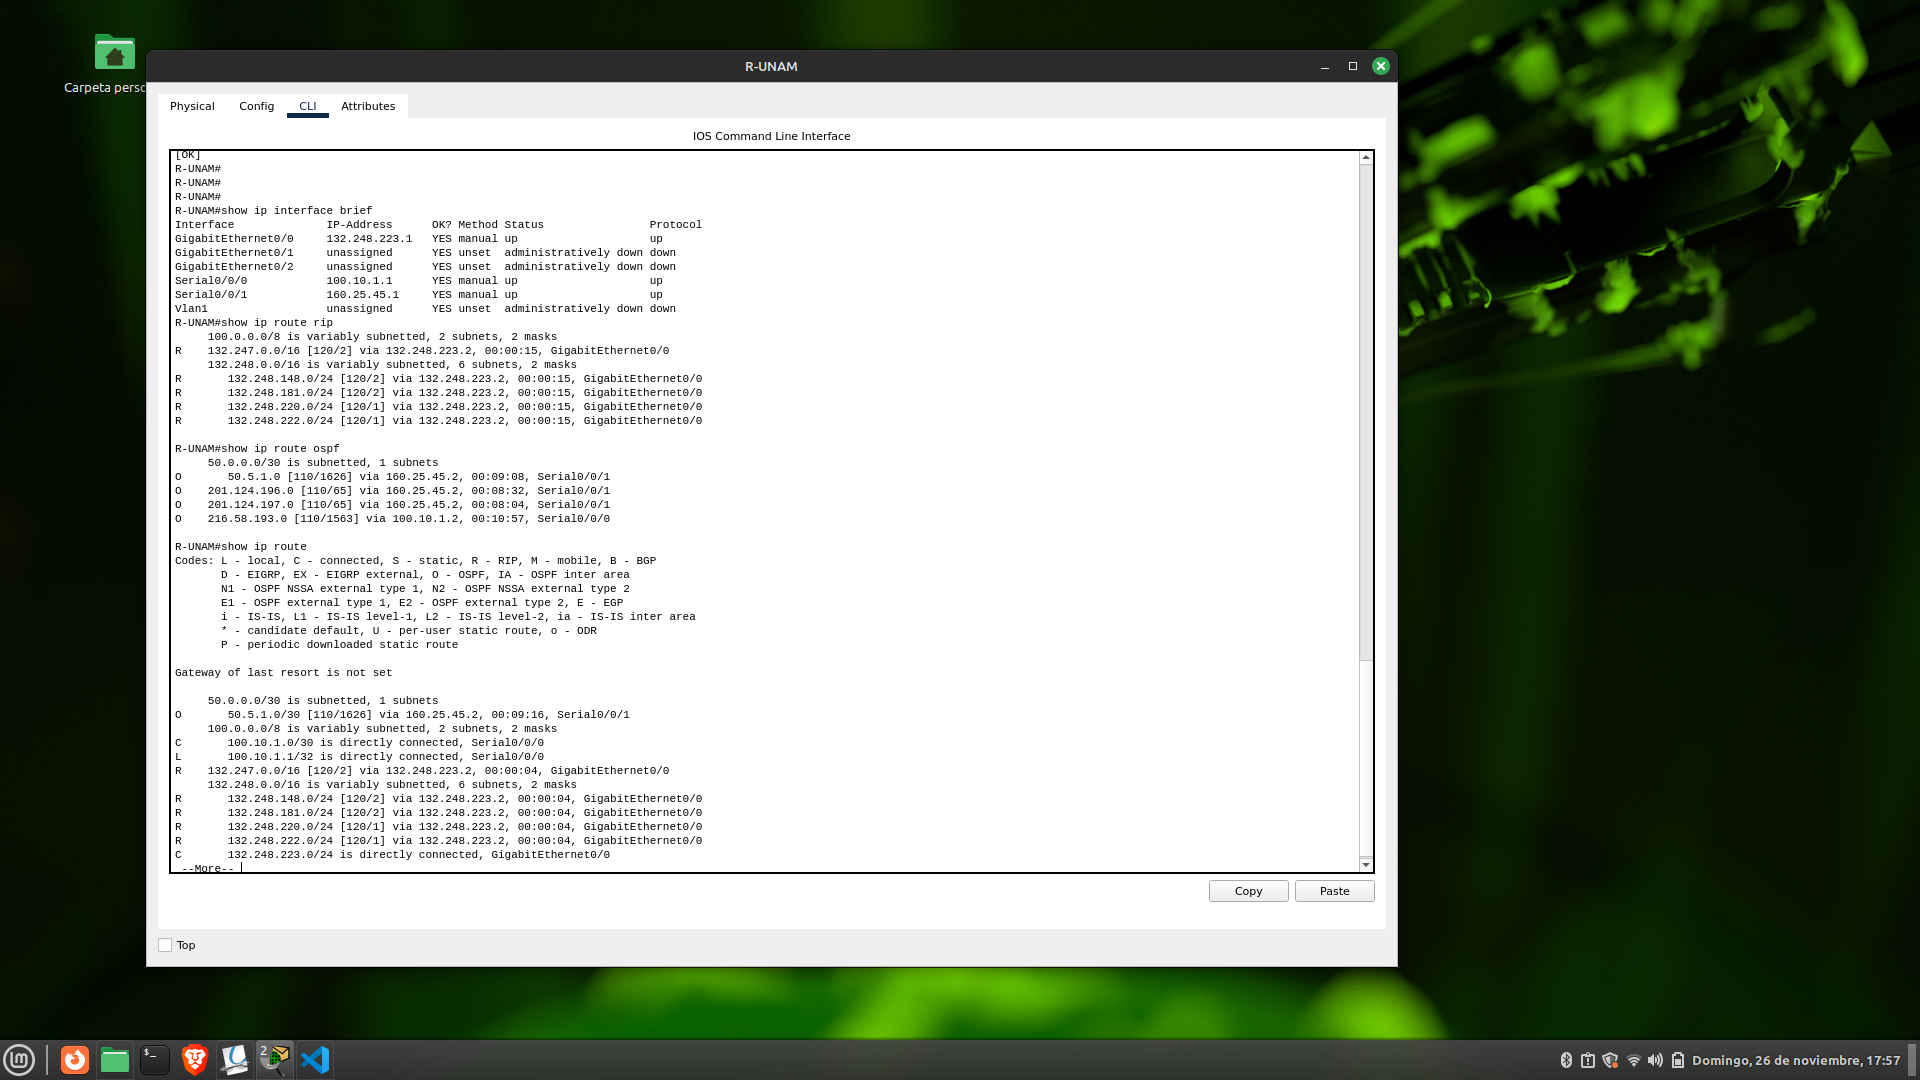
\includegraphics[width=12cm, height=8cm]{images/comandos UNAM.png}\\

Para Google:\\

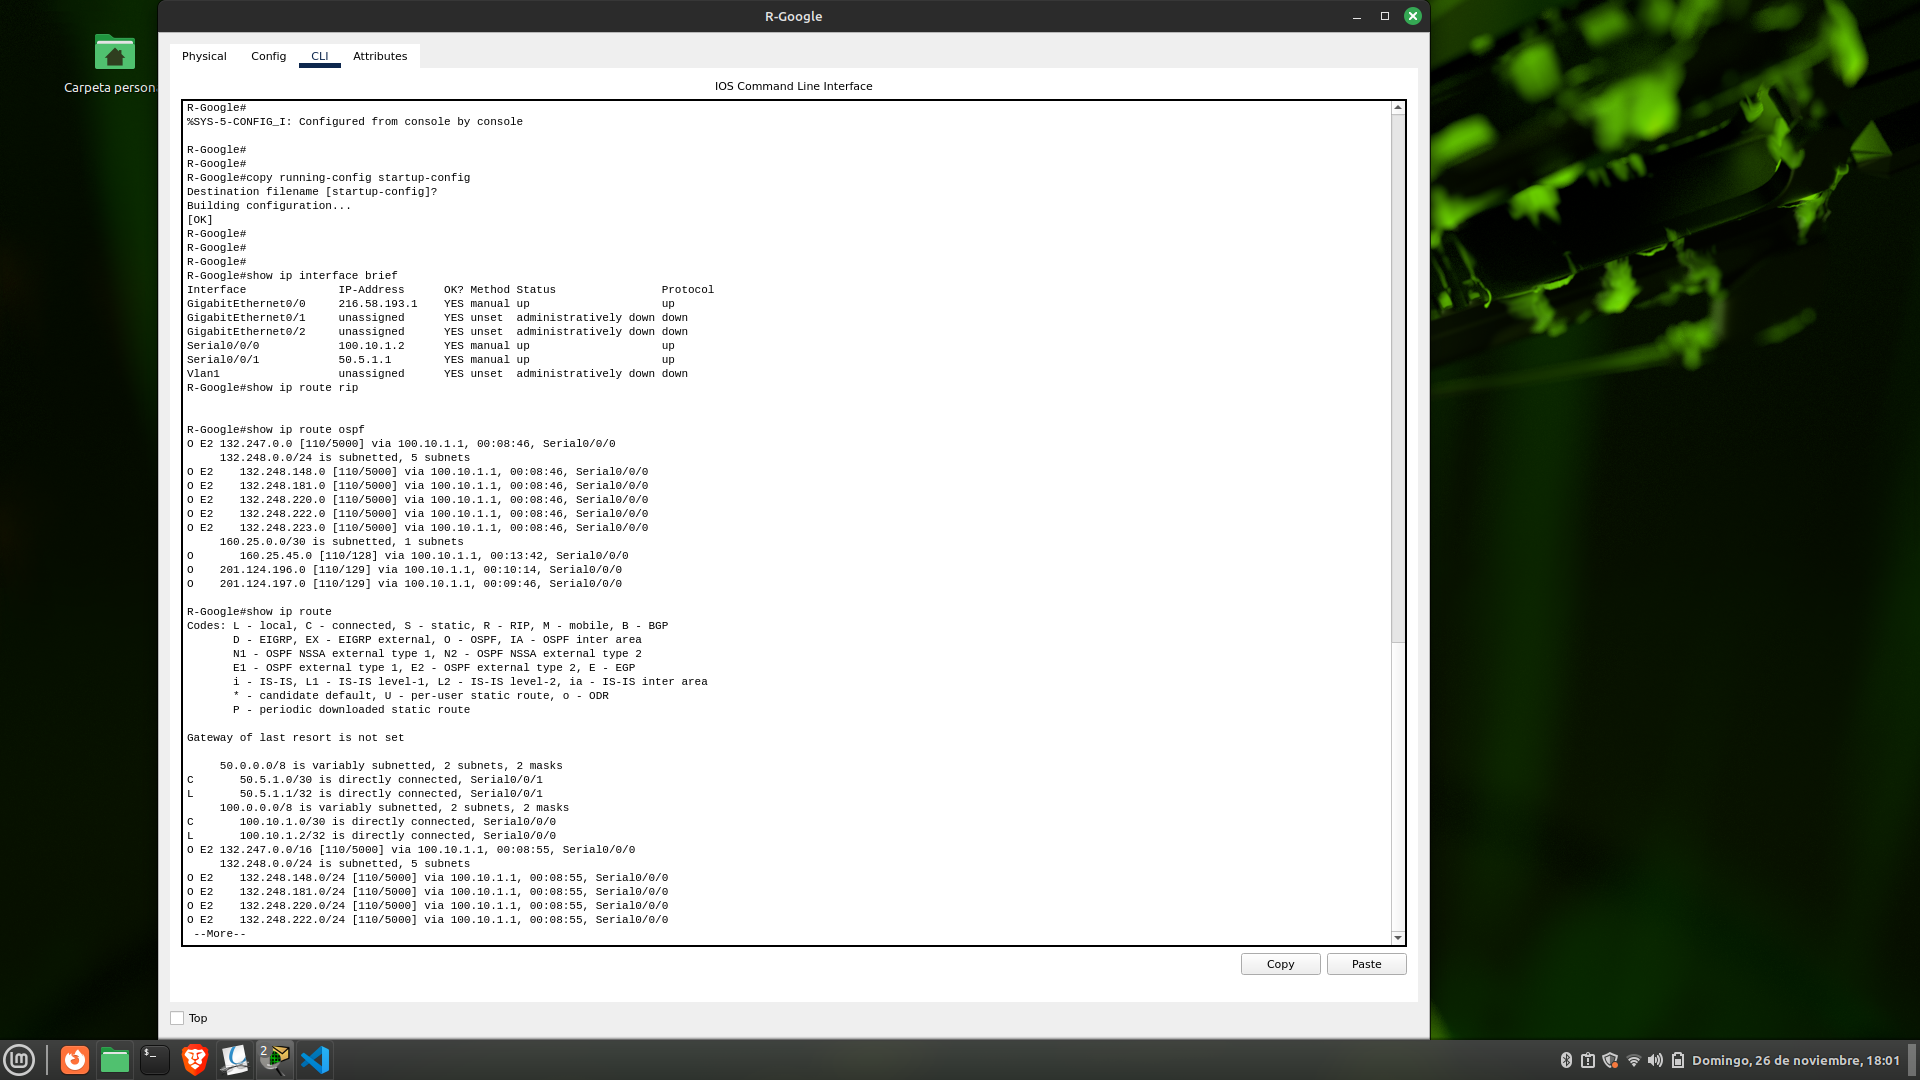
\includegraphics[width=12cm, height=8cm]{images/comandos GOOGLE.png}\\

Para Telmex:\\

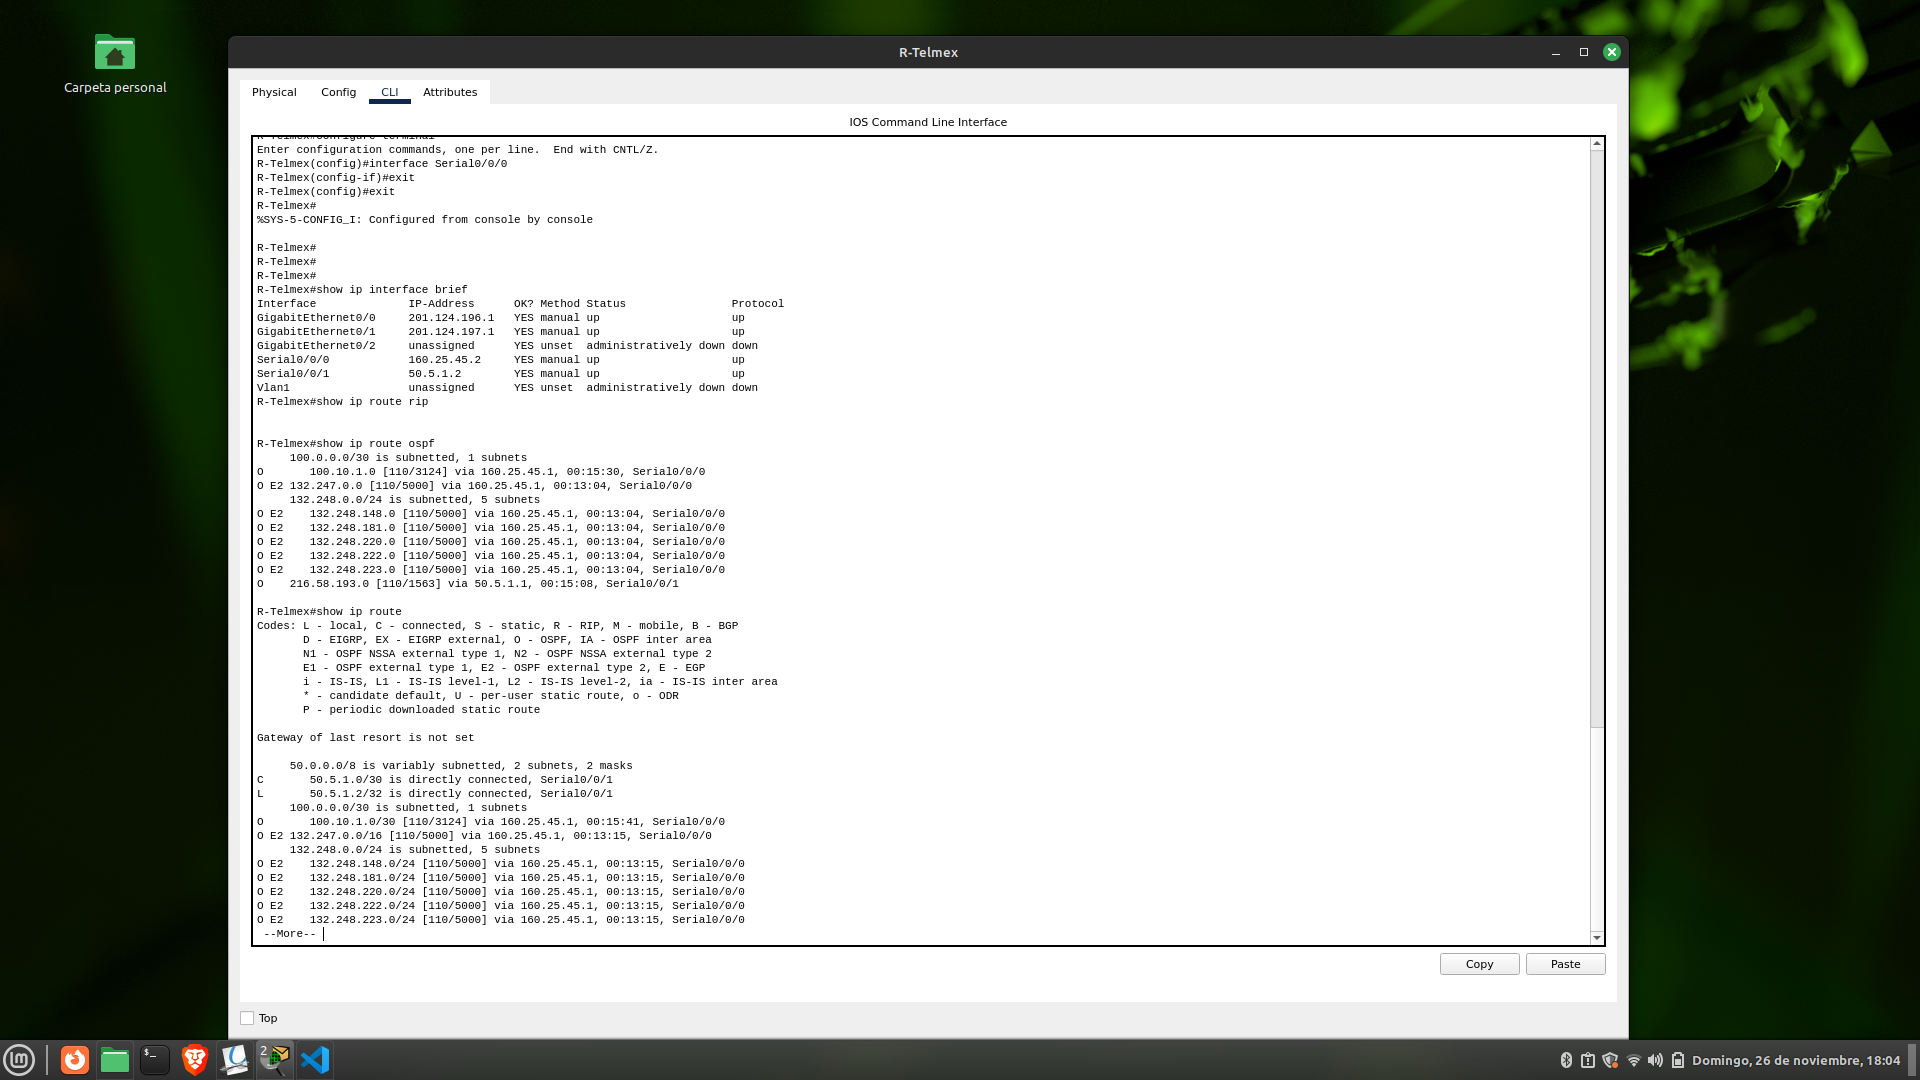
\includegraphics[width=12cm, height=8cm]{images/comandos TELMEX.png}\\

A continuación la explicación de los comandos:\\
\begin{enumerate}
  \item $Router show ip interface brief$: Este comando una muestra de la configuración y el estado de todas las interfaces IP en el router.
  \item $Router show ip route rip$: Este comando muestra la tabla de enrutamiento para el protocolo de enrutamiento RIP 
  \item $Router show ip route ospf$: Este comando muestra la tabla de enrutamiento para el protocolo de enrutamiento OSPF 
  \item $Router show ip route$: Este comando muestra la tabla de enrutamiento general del router, incluyendo todas las rutas aprendidas a través de varios protocolos de enrutamiento y las rutas estáticas configuradas.
\end{enumerate}

Acontinuación se ve las consultas a las paginas web:\\

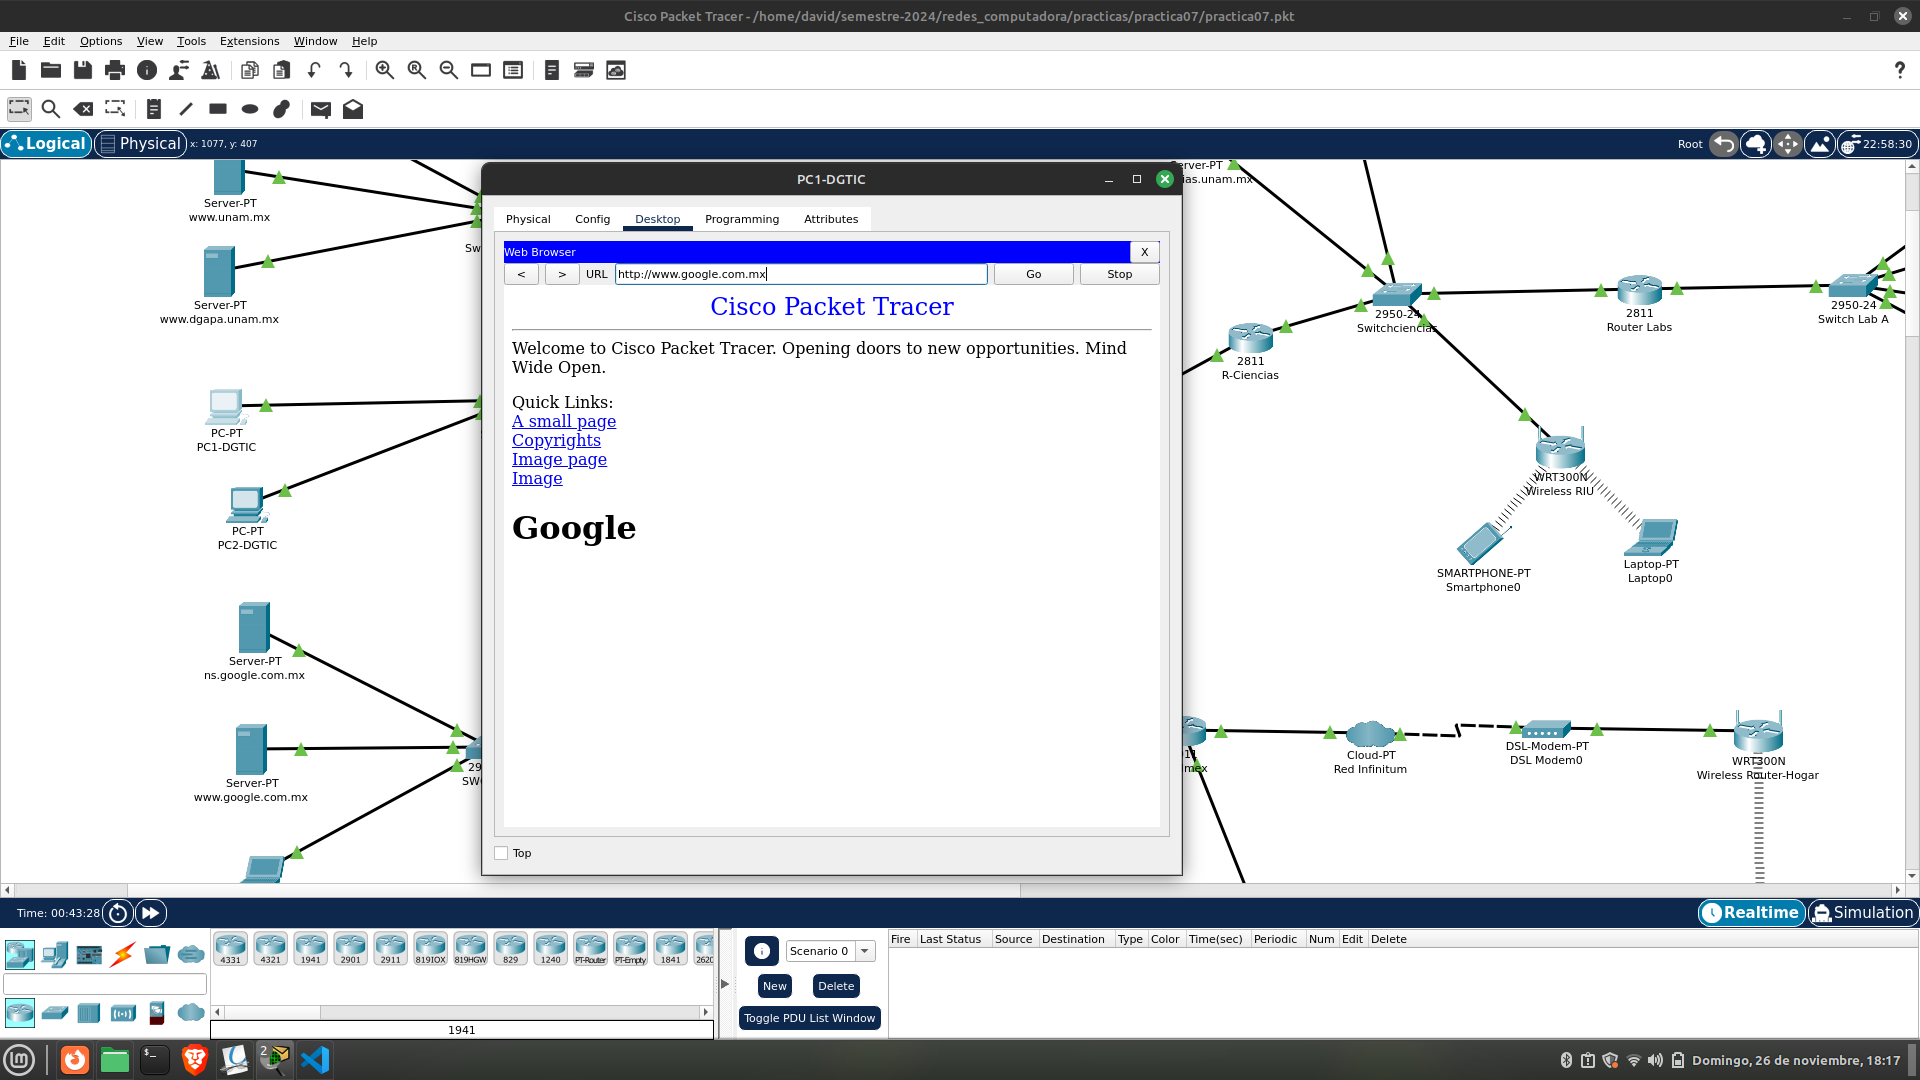
\includegraphics[width=12cm, height=8cm]{images/captura1.png}PC1-DGTIC a www.google.com.mx\\

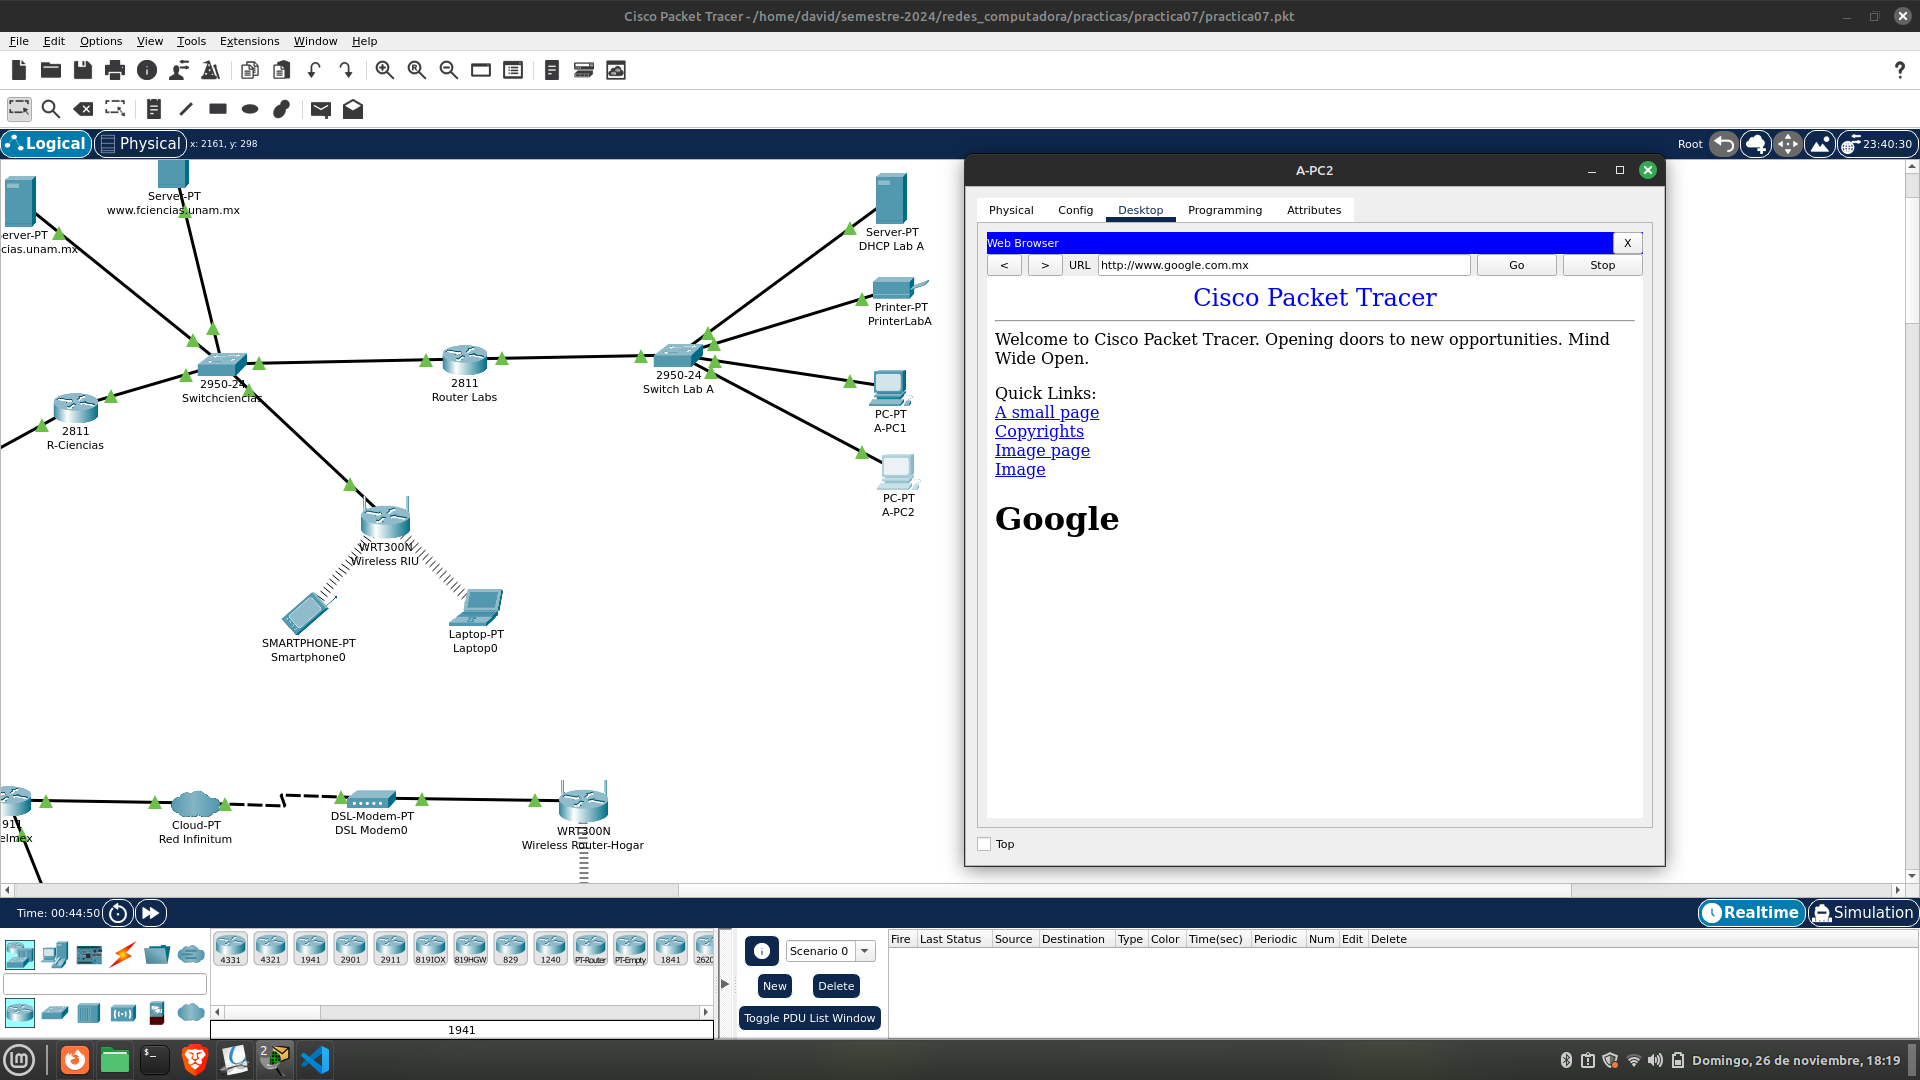
\includegraphics[width=12cm, height=8cm]{images/captura2.png}A-PC2 a www.google.com.mx\\

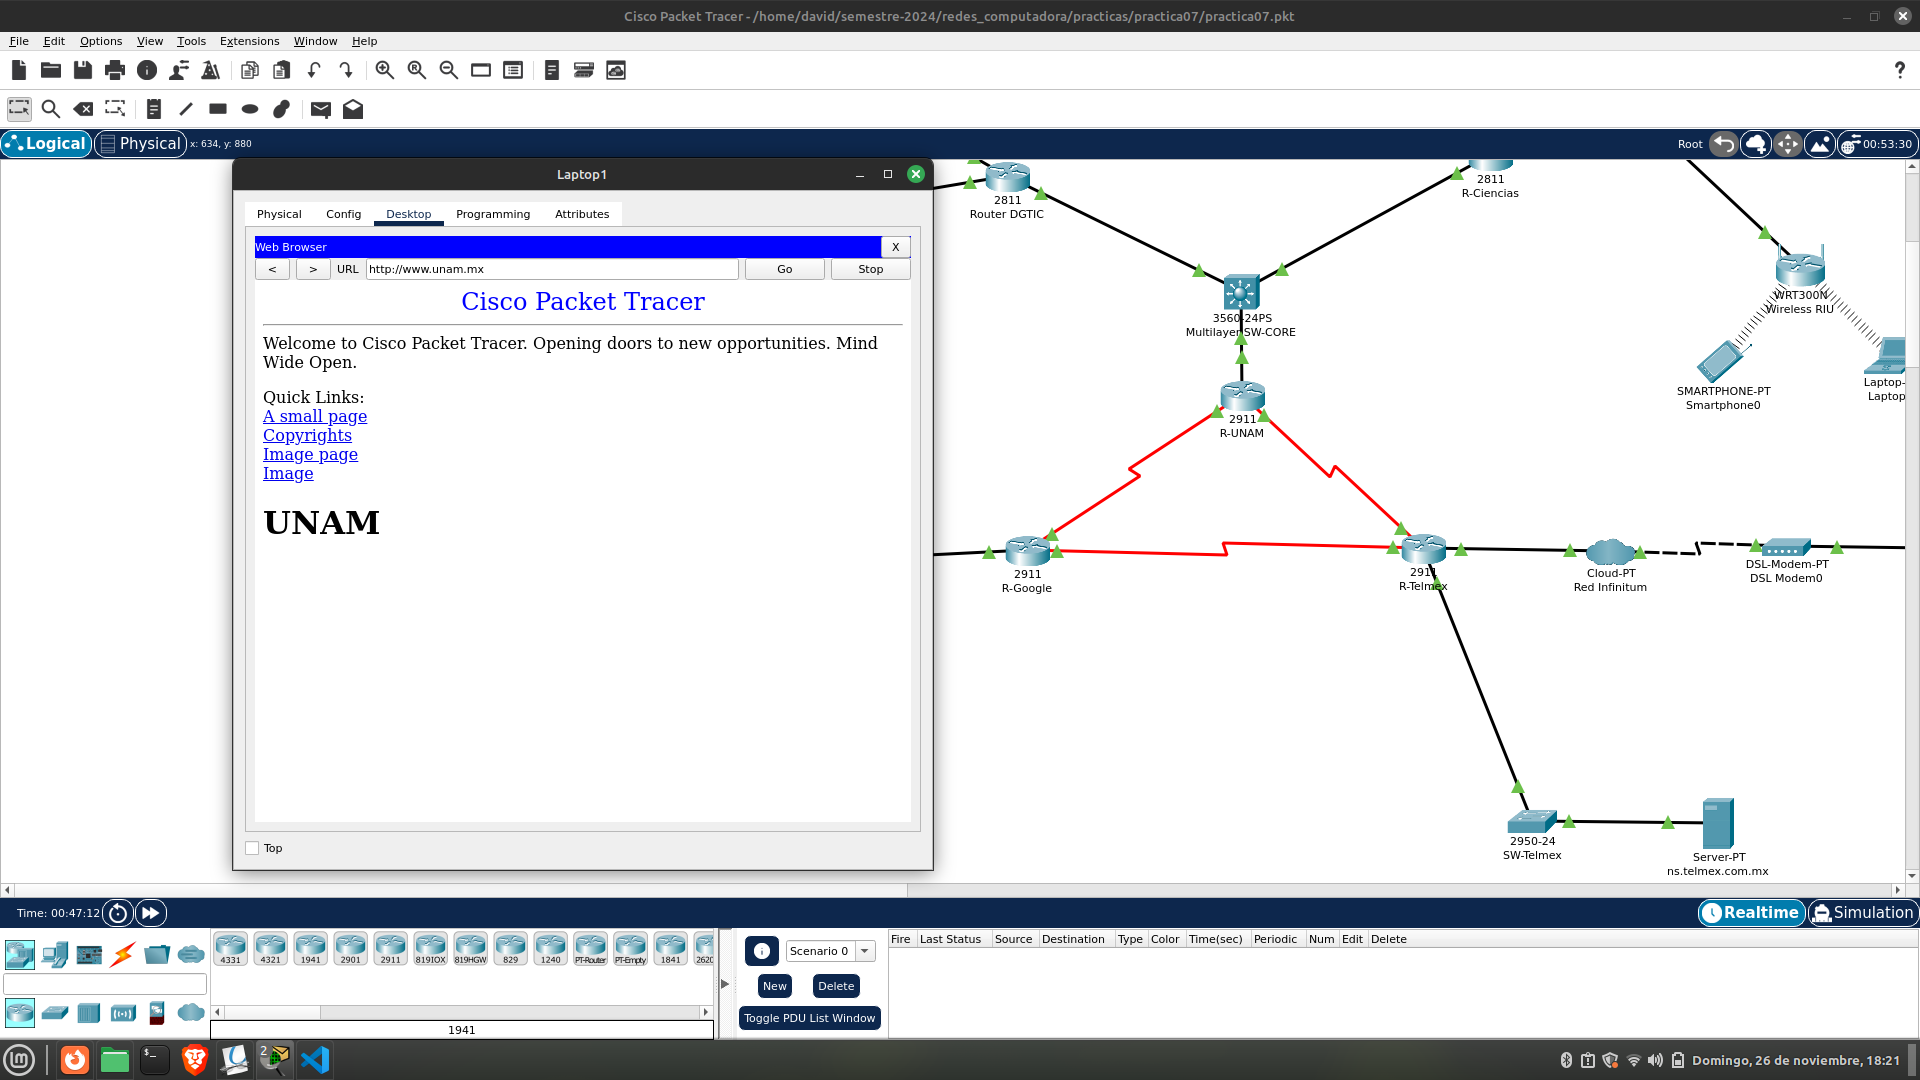
\includegraphics[width=12cm, height=8cm]{images/captura3.png}Laptop1 a www.unam.mx\\

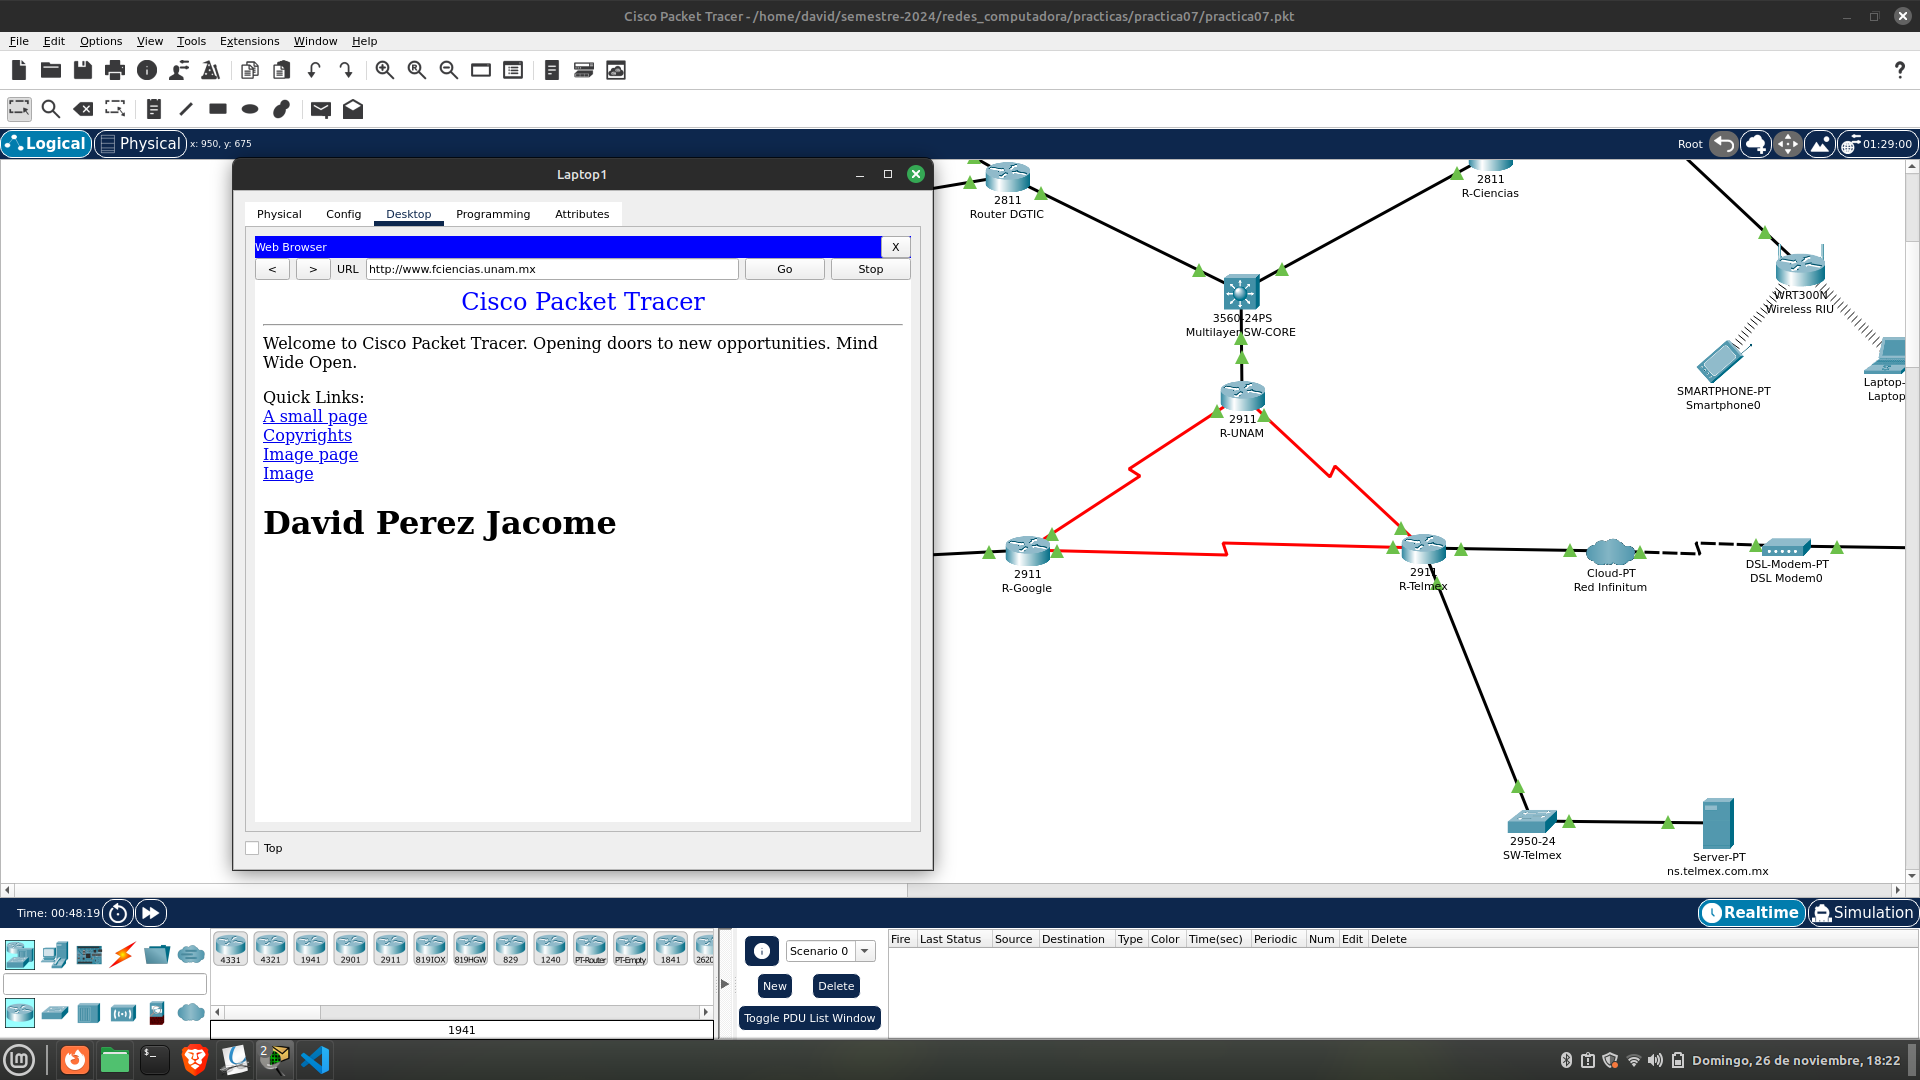
\includegraphics[width=12cm, height=8cm]{images/captura4.png}Laptop1 a   www.fciencias.unam.mx\\

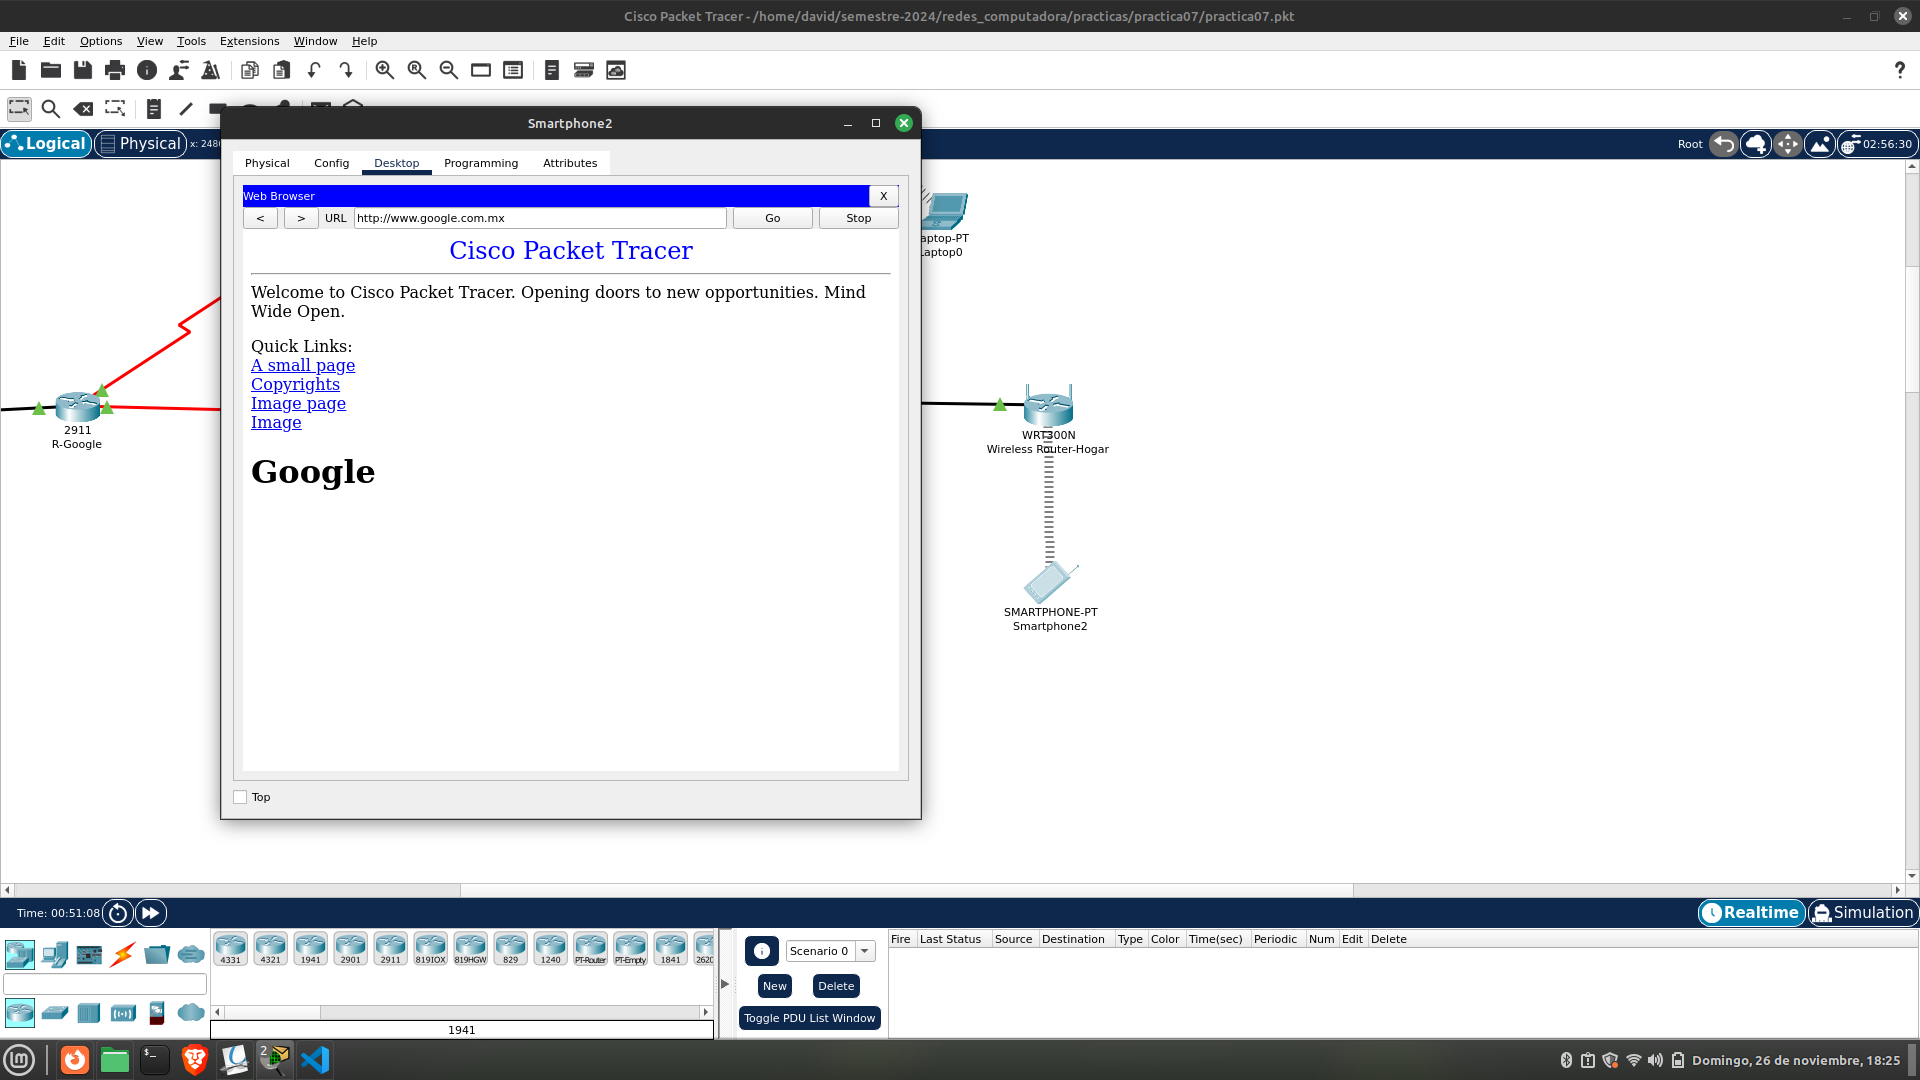
\includegraphics[width=12cm, height=8cm]{images/captura5.png}Smartphone2 a www.google.com.mx\\

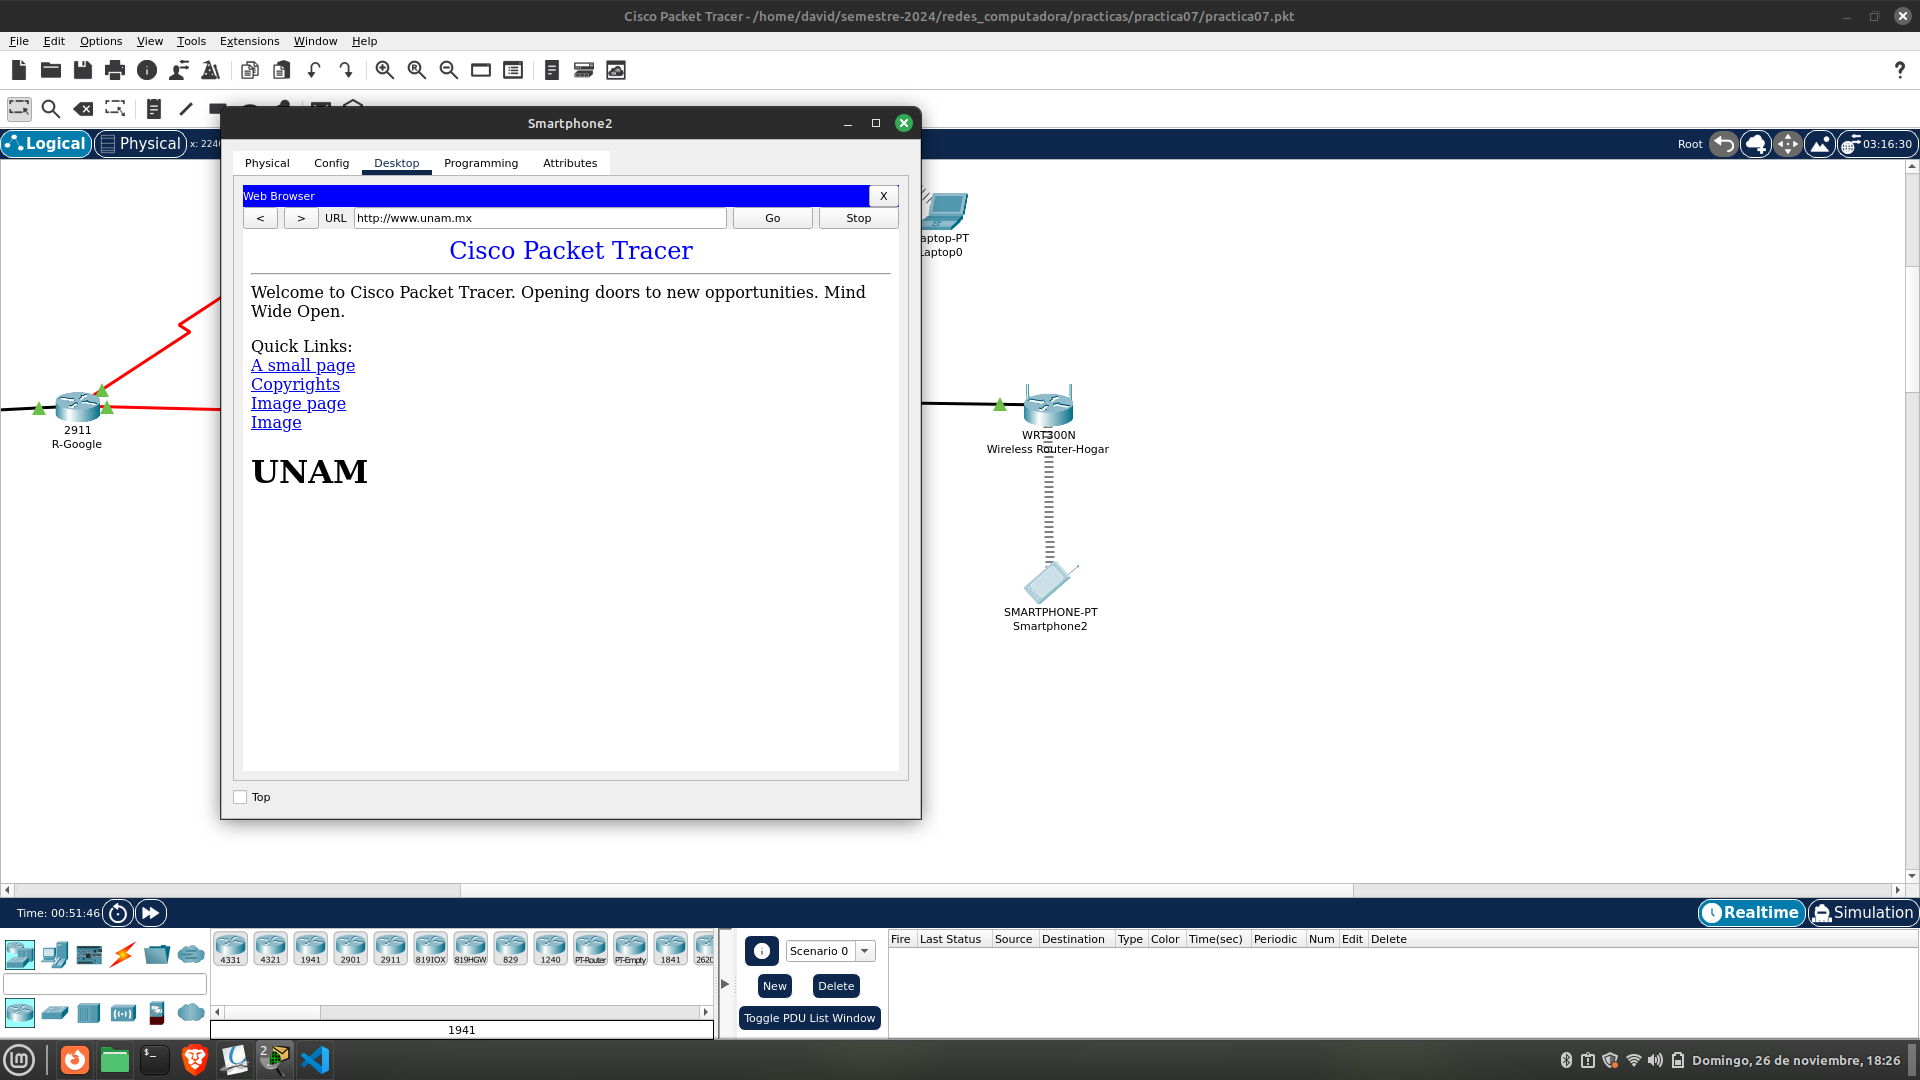
\includegraphics[width=12cm, height=8cm]{images/captura6.png}Smartphone2 a www.unam.mx\\

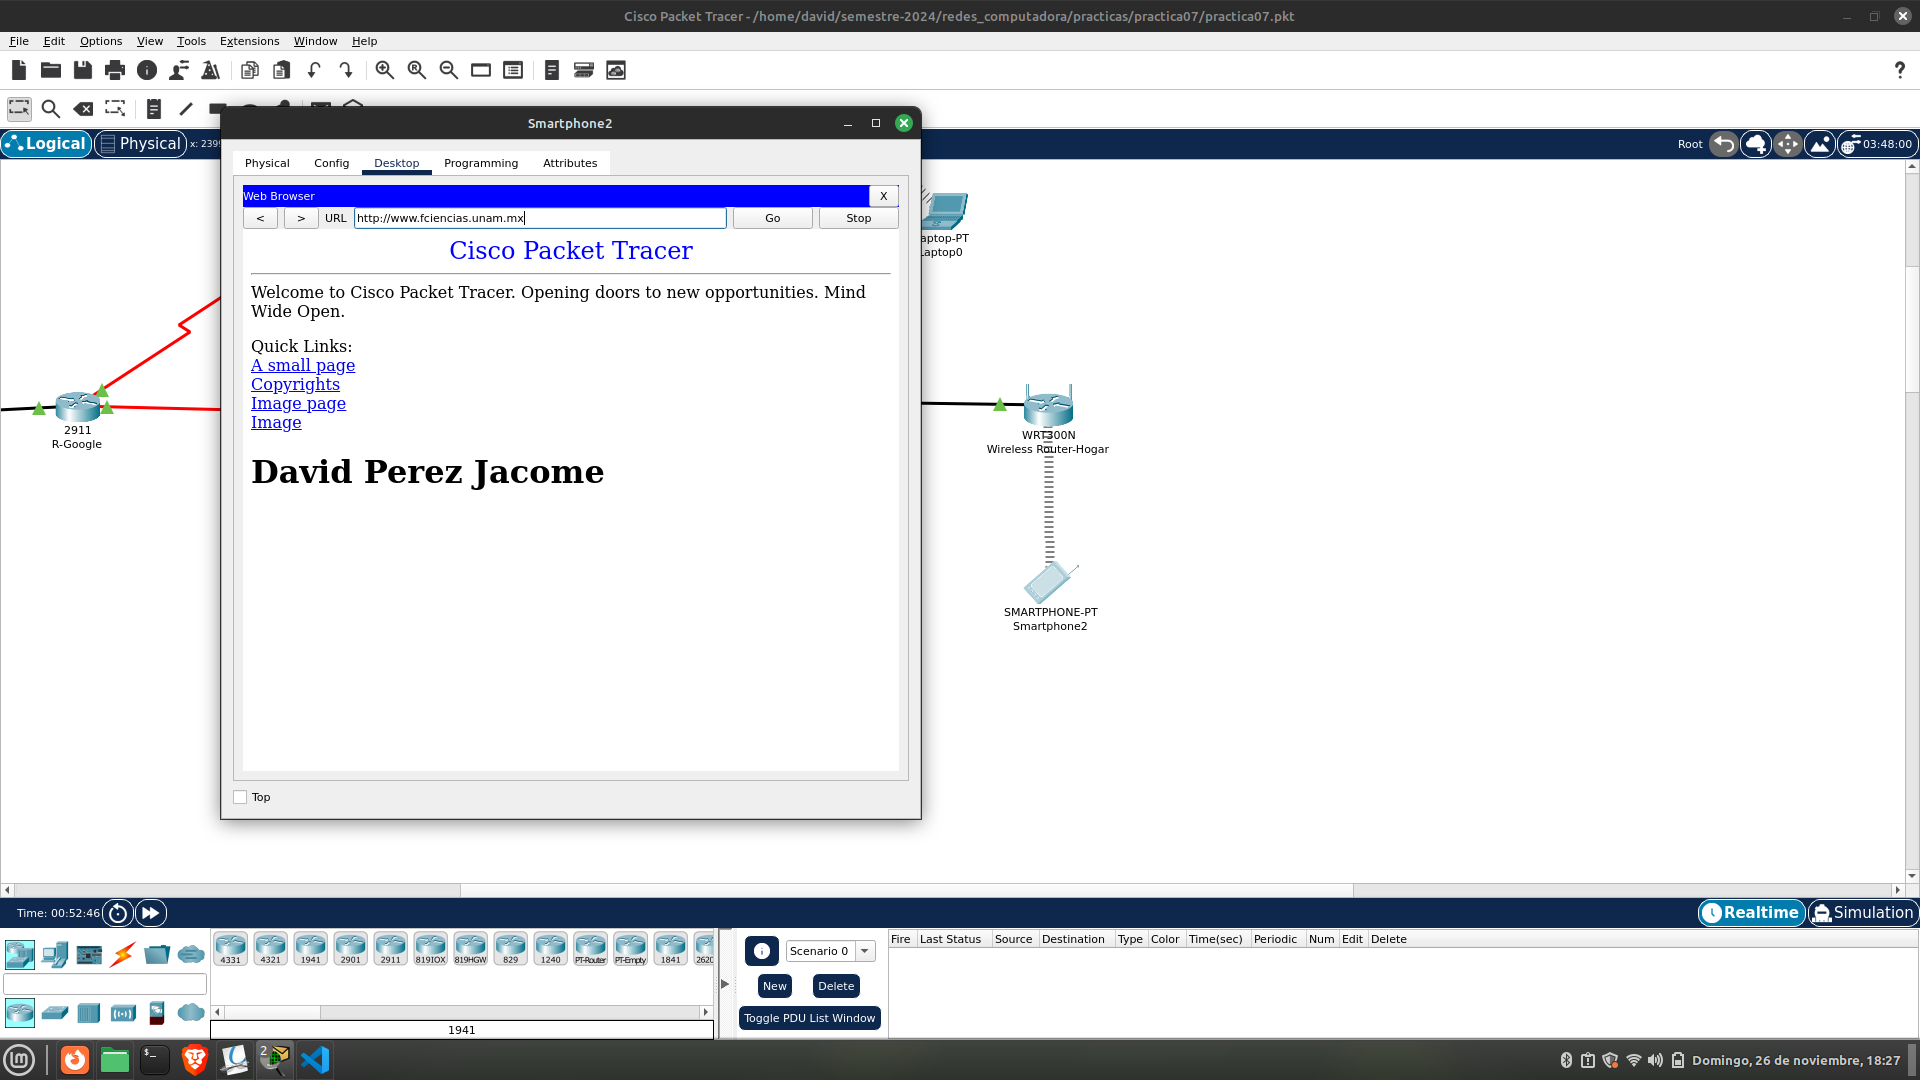
\includegraphics[width=12cm, height=8cm]{images/captura7 .png}Smartphone2 a www.fciencias.unam.mx\\

Mostraremos ahora la memoria caché de cada servidor DNS después de haber accedido a los sitios web.\\

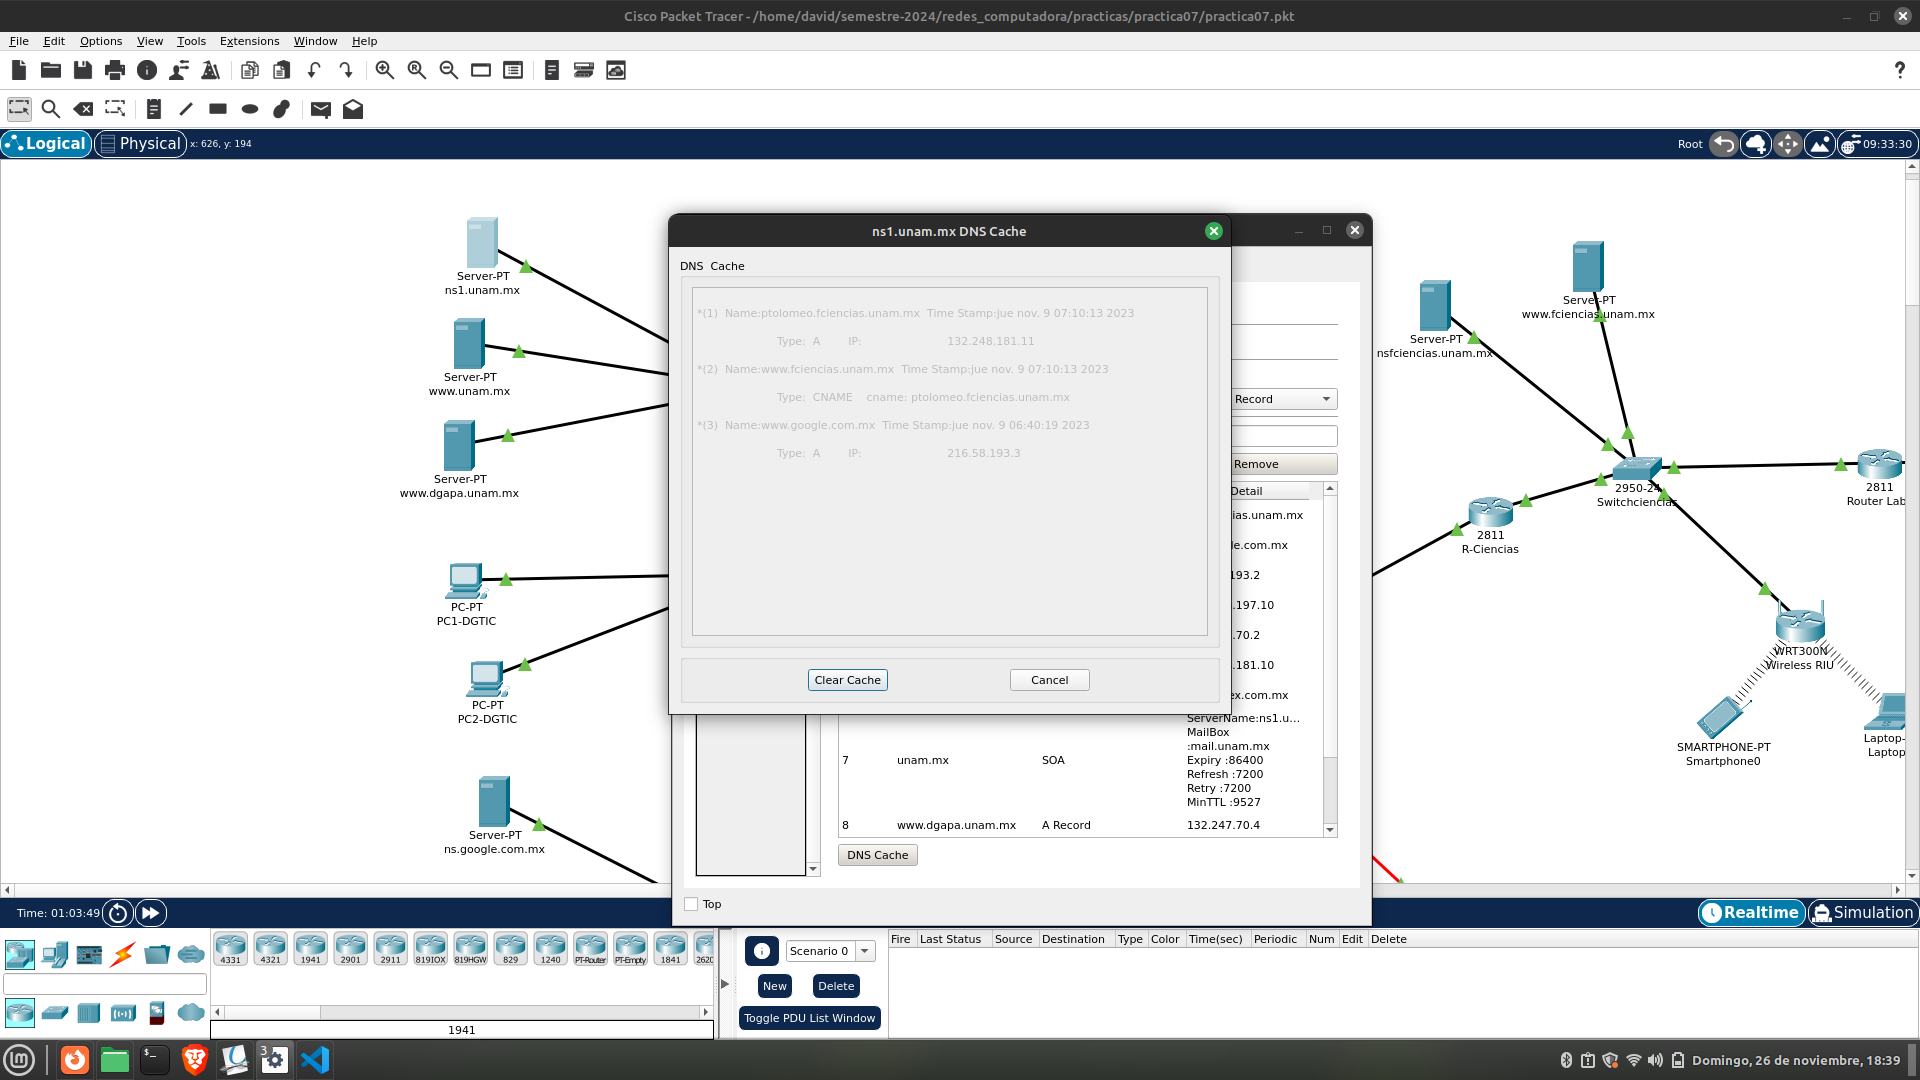
\includegraphics[width=12cm, height=8cm]{images/dns1.png}\\

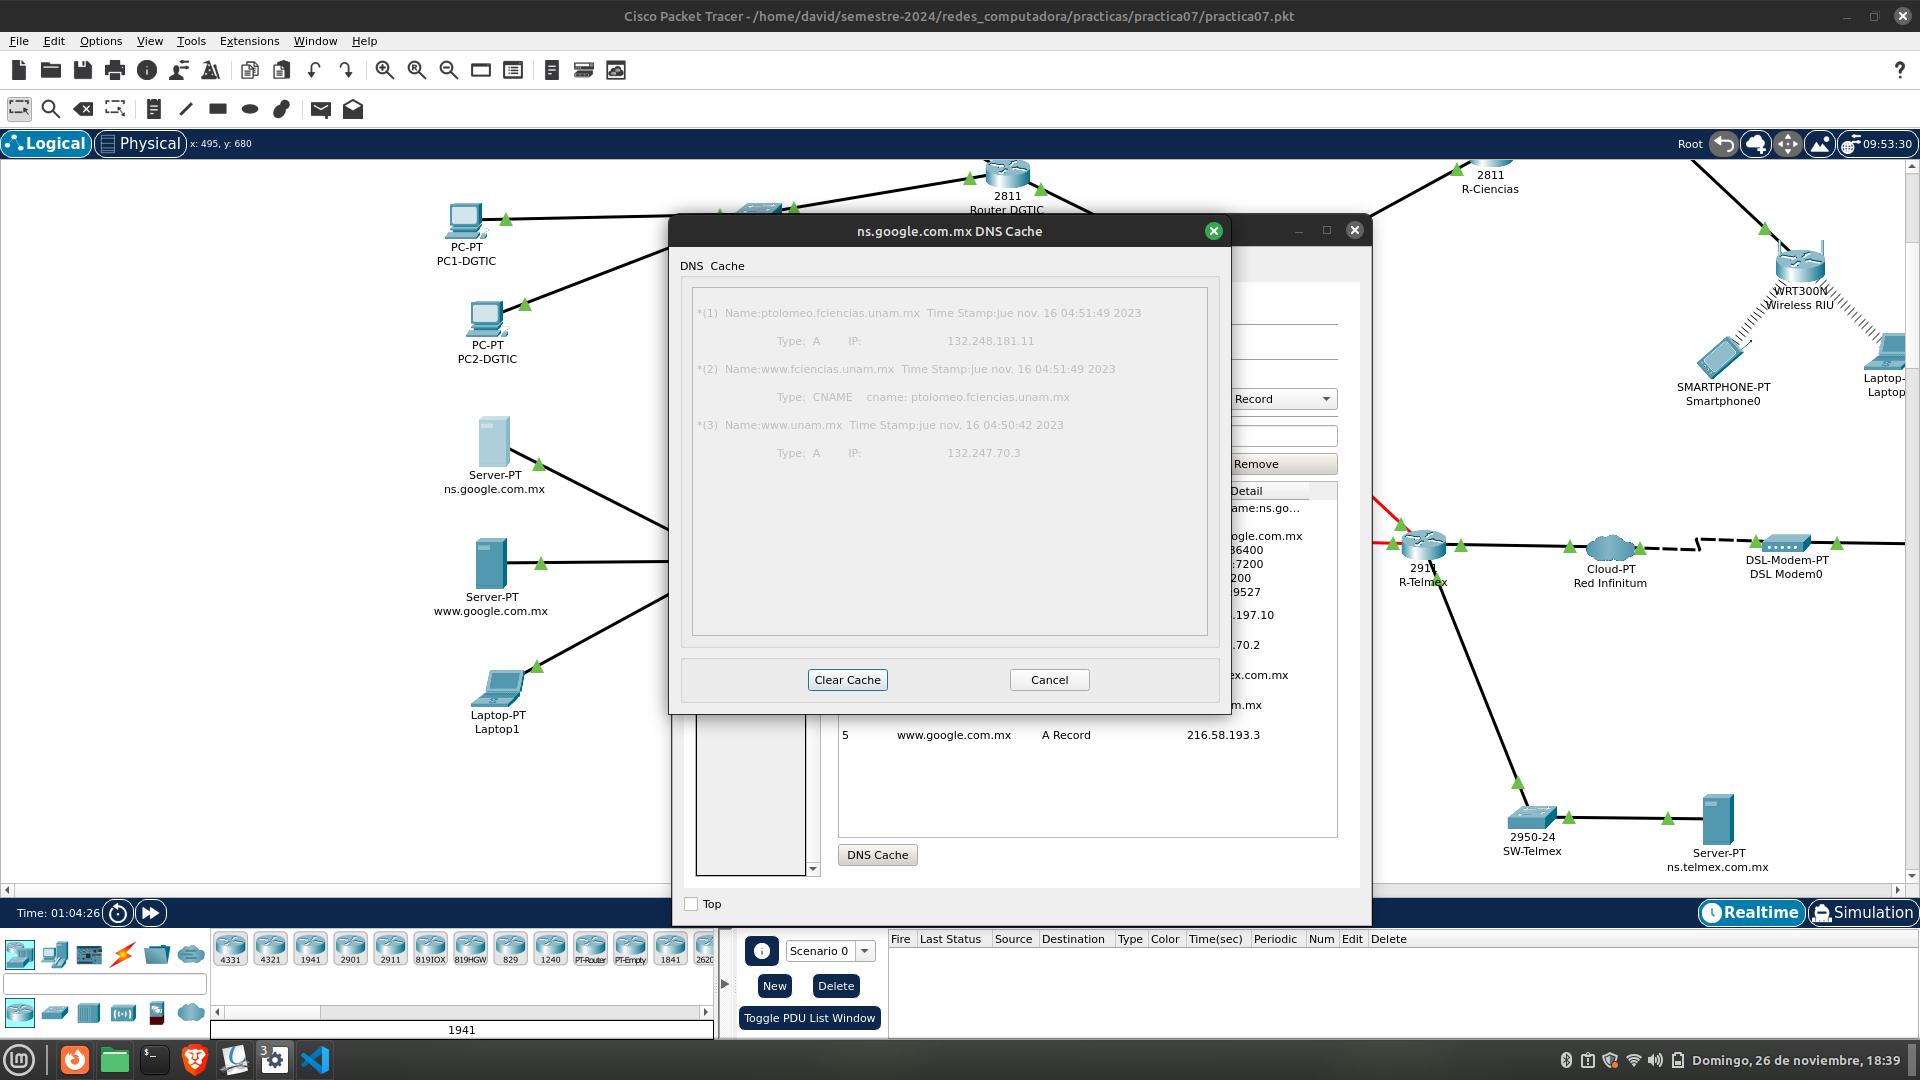
\includegraphics[width=12cm, height=8cm]{images/dns2.png}\\

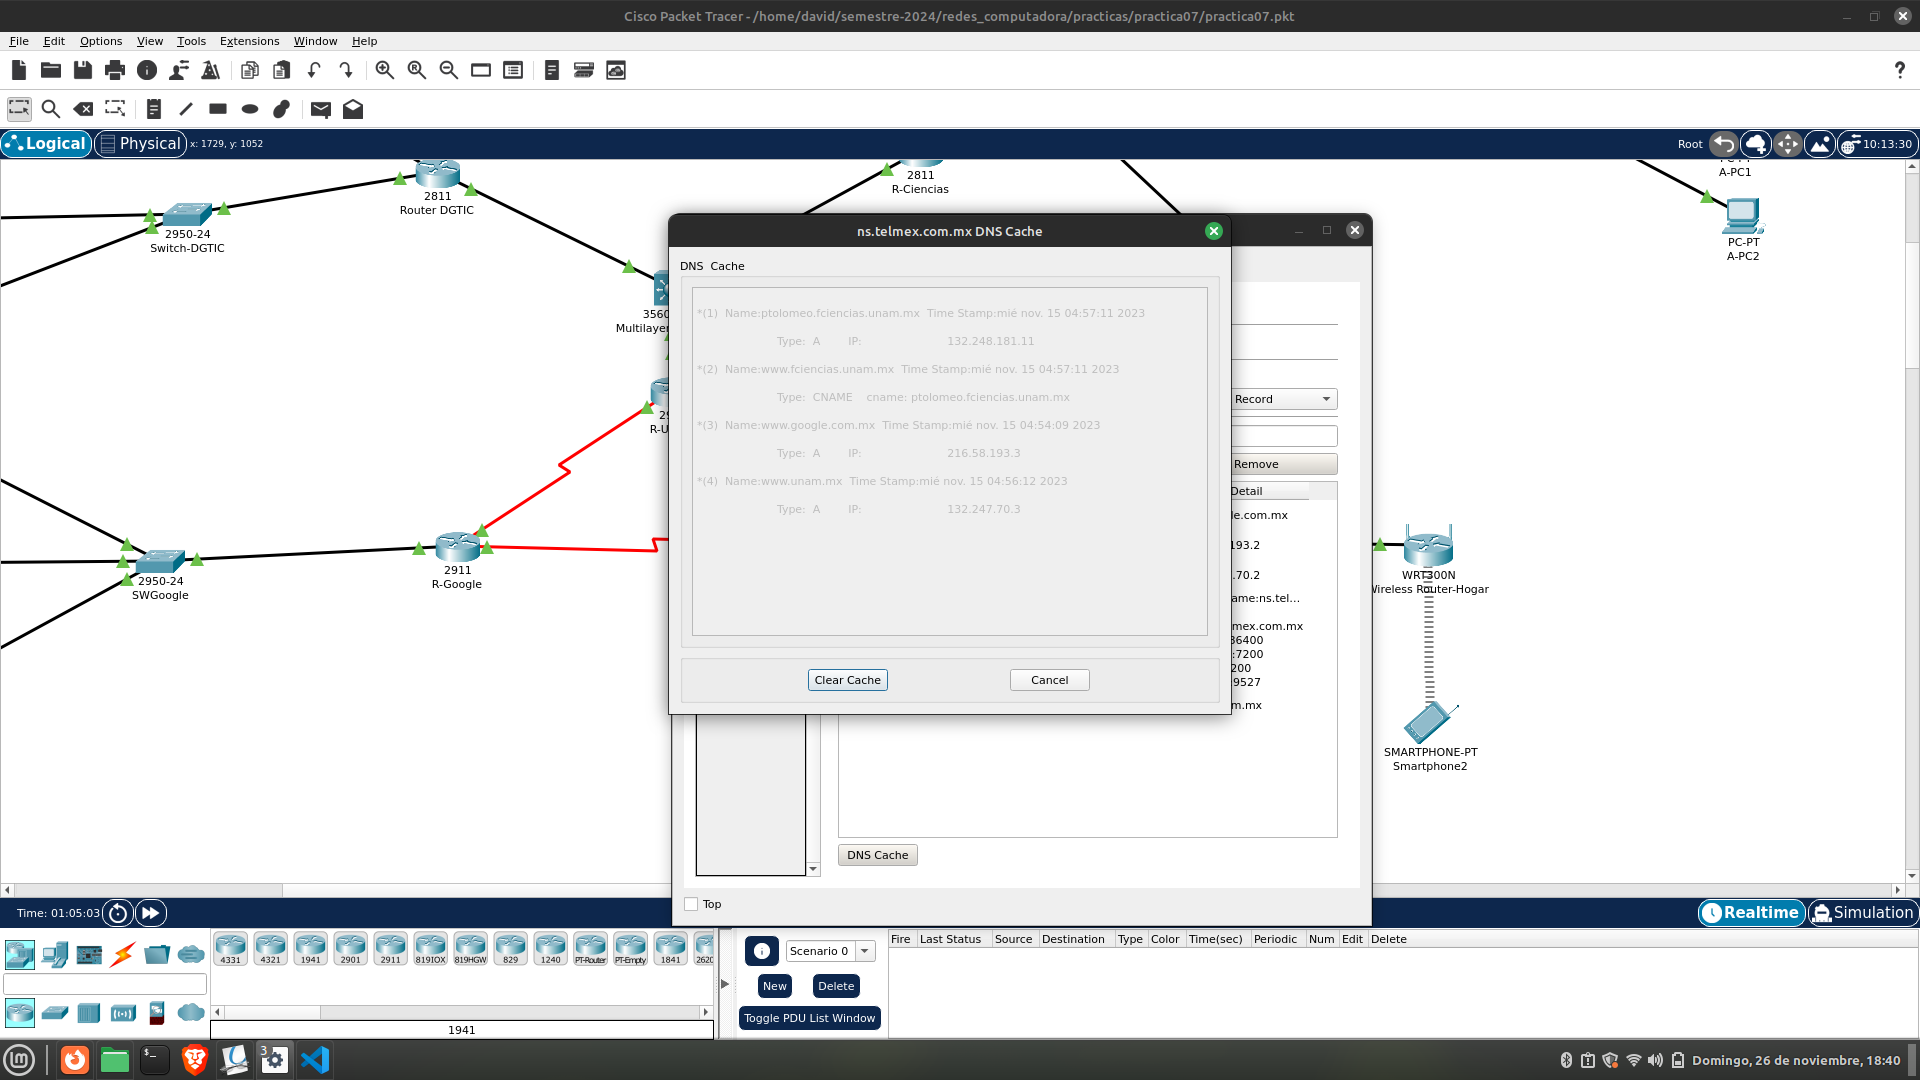
\includegraphics[width=12cm, height=8cm]{images/dns3.png}\\

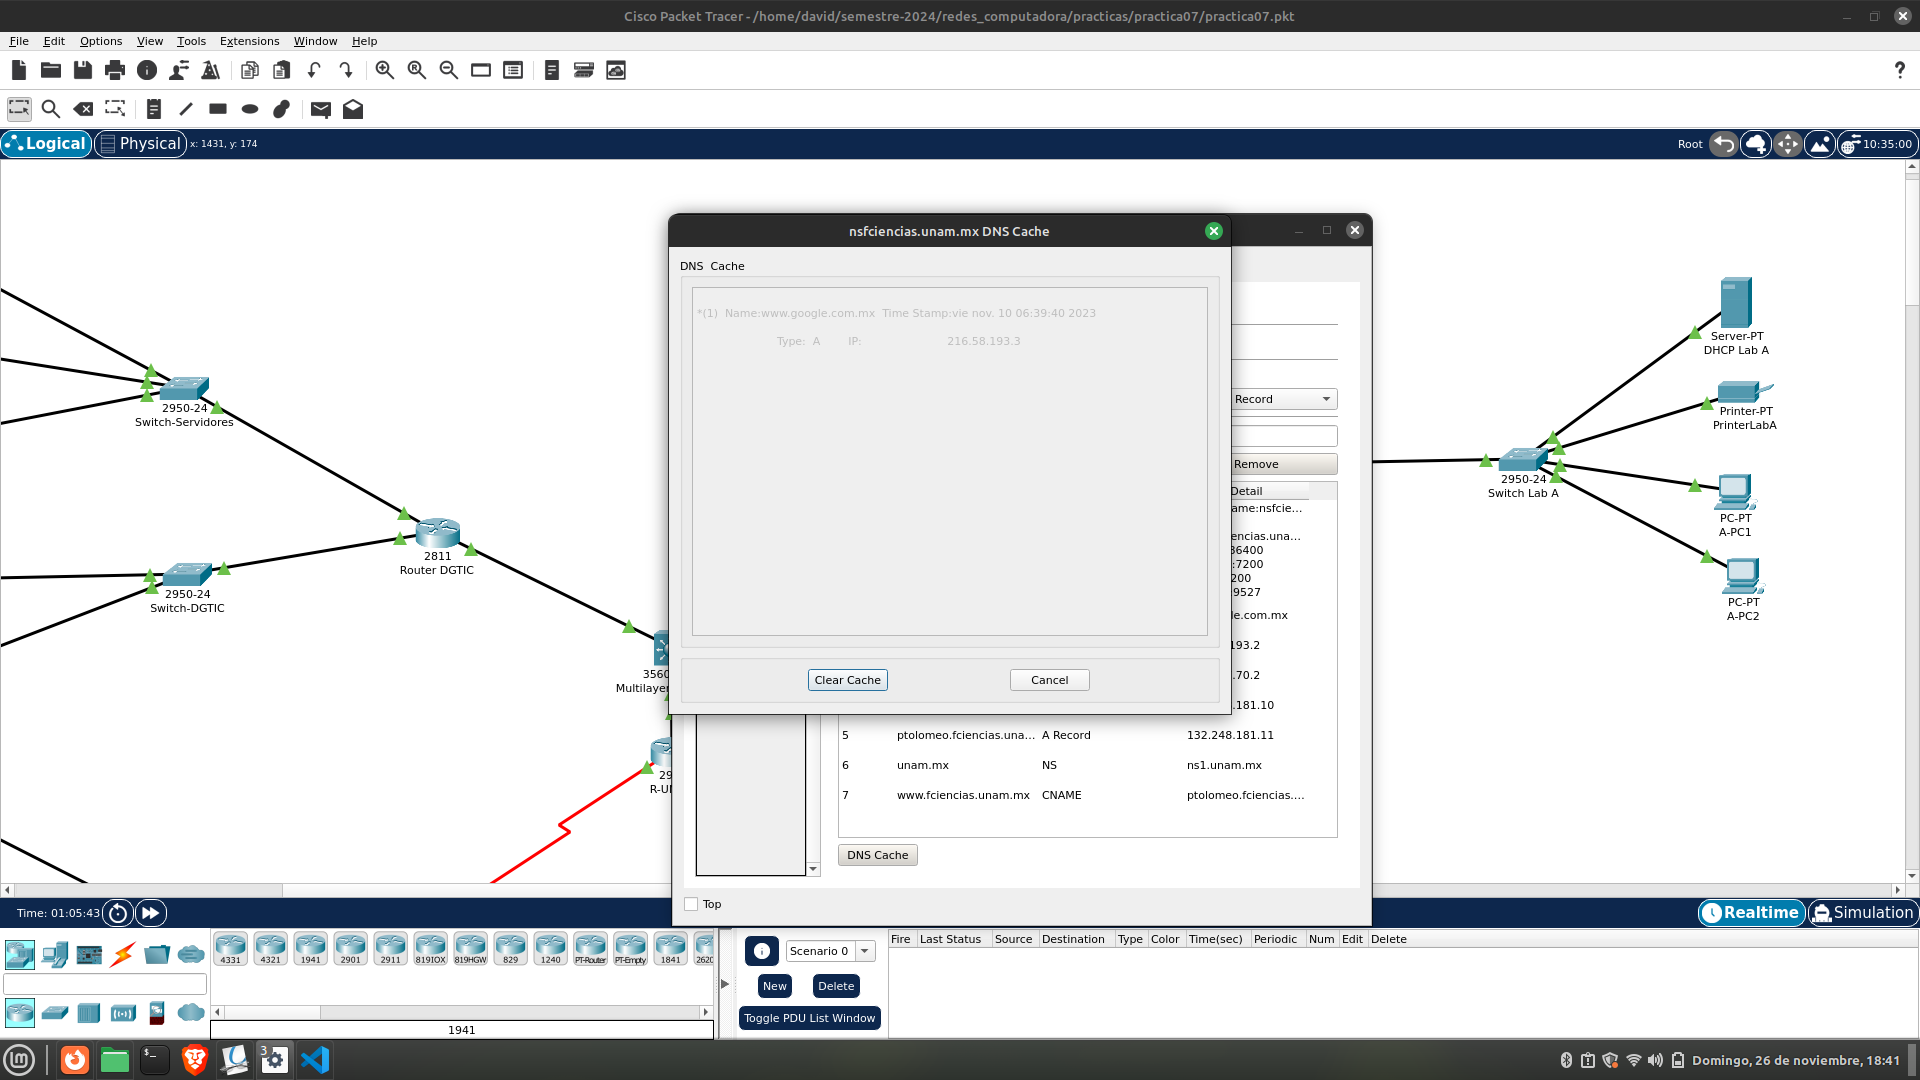
\includegraphics[width=12cm, height=8cm]{images/dns4.png}\\

{\color{blue} \subsubsection*{\textbf{Cuestionario}}}
\vspace{1em}

\begin{enumerate}
  \item ¿Qué algoritmo de ruteo implementa OSPF versión 2?\\
  \textbf{El algoritmo SPF se basa en la idea de construir un árbol de rutas desde el nodo de origen hasta todos los demás nodos en la red, utilizando la información de costo asociada con cada enlace. OSPF utiliza este enfoque para construir su base de datos topológica y calcular las rutas más cortas para cada destino en la red. }
  \item ¿Cuáles son las diferencias entre los protocolos de ruteo de interdominio y los protocolos de ruteo intradominio?\\
  \textbf{la principal diferencia radica en el alcance de aplicación: los protocolos de ruteo de interdominio se utilizan para rutas entre diferentes dominios autónomos (por ejemplo, en Internet), mientras que los protocolos de ruteo de intradominio se utilizan para rutas dentro de un único dominio autónomo (como una red corporativa).}
  \item  ¿Qué tipo de protocolo de ruteo, interdominio o intradominio, son RIP y OSPF?\\
  \textbf{RIP (Routing Information Protocol) y OSPF (Open Shortest Path First) son protocolos de ruteo intradominio, también conocidos como protocolos de ruteo interno.}
\end{enumerate}



\end{document}